%-A Two-Qubit Quantum Processor
%-Building Blocks: Single Qubit Gates, Qubit Readout, Two-Qubit Gate
%-Implementation
%-Frequency Tunability of the Qubits
%  -Decoherence Times
%-Characterization of the Readout
%  -Readout Errors
%-Single Qubit Gates: Tune-Up & Characterization
%-2 Qubit Gate: Tune-Up & Characterization
%-Tests of Entanglement
%  -Entanglement Witnesses
%  -Bell's Inequality
%-2 Qubit Algorithms
%-Grover's Search Algorithm:
%   -Introduction & Background
%   -Implementation
%   -Measurements
%   -Error Analysis
%   -Conclusions

\chapter{Realizing a Two-Qubit Processor}

This chapter discusses the main experimental results of this thesis. We start by discussing the implementation of a superconducting two-qubit processor, discussing the characteristics of the Transmon qubits used in the processor, the readout scheme, single-qubit manipulation, two-qubit gates as well as the experimental procedures used for quantum state and quantum process tomography. The last section of this chapter will discuss the implementation of a quantum algorithm -- so called Grover search algorithm -- using our two-qubit processor and the demonstration of quantum speed-up achieved with our system.

%-Discuss all the experiments performed during the PhD thesis.

\section{Introduction \& Motivation}

\begin{figure}[ht!]
  \centering
	\includegraphics[width=1.\textwidth]{"./material/figures/2-qubit-processor/processor schematic"}
	\caption[Circuit schematic of the two-qubit processor]{The circuit schematic of the two-qubit processor used in this work. Shown are the two Transmon qubits in green, the drive and readout circuit in blue, the fast flux lines in red and the coupling capacitance in magenta.}
	\label{fig:2_qubit_chip_circuit_diagram}
\end{figure}

As discussed in the introduction, the most simple, usable quantum processor contains two qubits that are coupled by an universal two-qubit gate and which in addition can be manipulated and read out individually. We realized such a two-qubit processor using two Transmon qubits, coupled through a fixed capacitance and readout out by individual single-shot readout of the JBA type. The circuit diagram of our processor is shown in fig. \ref{fig:2_qubit_chip_circuit_diagram}, showing the qubits, the drive and readout circuit and the coupling element between them. The following sections we'll discuss the parameters of individual parts of the processor.

\section{Qubit Design}

The parameters of the sample have been chosen in accordance to various design constraints of the qubit processor. For the qubits, the main design goals were high coherence time, good frequency tunability and fast drivability. As we will show later, the coherence time of the qubit is limited by relaxation to the ground state and coupling to external noise sources. The relaxation component of the Transmon qubit is ultimately limited by internal losses of the Josephson junction but usually is bound by coupling to the electromagnetic environment, as will be discussed later. The frequency tunability is important for the realization of fast two-qubit gates but can also limit the relaxation and coherence time of the qubit by coupling to external noise sources. The drivability speed on the other hand is limited by the anharmonicity of the qubit, which can however not be increased arbitrarily since it will make the qubit sensitive to charge noise when chosen too high. For the readout, the main design goals were readout speed and fidelity. The speed of the readout is limited by the quality factor of the readout resonator, which however also can induce qubit relaxation through the Purcell effect and may therefore not be chosen too small.

In the following paragraphs we'll therefore discuss the parameter design for our two-qubit processor and analyze the sample parameters that have been obtained.

\section{Readout Design}

\section{Processor Fabrication}

In this section we will discuss the fabrication of the two-qubit processor realized in this work.

\chapter{Measurement Setup}

\begin{figure}[ht!]
	\centering
		\includegraphics[width=1.\textwidth]{"./material/figures/2-qubit-processor/measurement setup"}
	\caption[The measurement setup used for the two-qubit experiments]{The measurement setup used for the two-qubit experiments. Exactly the same drive and readout scheme is used for both qubits with phase-locked microwave sources and arbitrary waveform generators.}
	\label{fig:MeasurementSetup}
\end{figure}

Fig. \ref{fig:MeasurementSetup} show the measurement setup used for the two-qubit experiments. The different signal and measurement lines as well as the room-temperature and cryogenic microwave components used in our experiments will be described in the following paragraphs.

In this section we discuss the details of the measurement setup used to perform the two-qubit experiments presented in this thesis. All experiments have been performed in a custum-built dilution cryostat at $< 40 \; \mathrm{mK}$ using a cryogenic microwave signal generation and measurement chain. The individual components of this setup will be discussed in the following sections.

\section{Sample Holder \& PCB}

The qubit chip is first glued to a high-frequency PCB \todo{add substrate material details}, then wirebonds are used to connect the groundplane and the center conductors of the on-chip transmission lines to their counterparts on the PCB. Finally, additional bond wires connect isolated ground planes on-chip. The realization of a good and uniform groundplane on the qubit chip and around is very important to supress unwanted resonance modes that can be created when the connection between isolated ground planes is not good enough \todo{Add references e.g. to Schuster's thesis}. The mounted chip on the PCB is then placed in a Copper or Aluminium sample holder which fully encloses the PCB and serves to reduce unwanted couplings to the environment. The coplanar waveguides on the PCB are connected to Mini-SMP cables through a set of connectors that are soldered on the PCB.

\section{Cryogenic Wiring}

For the transmission of microwave signals to our sample we use various types of transmission lines suited for room-temperature and cryogenic application. The main goal of the input lines is to provide adequate signal transmission without introducing too much thermal conductance to the system. For the signal lines that carry the measurement signal from the sample we use superconducting cables \todo{add type} and low-resistance copper cables. In addition, we use superconducting bifilar cables for the DC bias of our magnetic coils. The qubit and fluxline input lines are attenuated and filtered at several stages of the cryostat to reduce signal noise.

\section{Signal Generation \& Acquisition}

Here we discuss the generation and acquisition of the different signals used to manipulate and read out our quantum processor. The experiments that have been performed require the generation, measurement and demodulation of microwave signals, the generation of fast flux control pulses and the application of DC currents to our magnetic coils.

\subsection{Microwave Sideband Mixing}

For qubit manipulation it is often advantageous to use single-sideband mixing for driving the qubit since it can provide higher ON/OFF ratios for microwave pulses and allow the driving of higher qubit-levels using a single, phase-coherent microwave source. To realize this, we use IQ mixers (Hittite \todo{Add exact type number}) that we drive with a continous single-frequency microwave tone and two time-synchronized fast control signals generated by an arbitrary waveform generator (Tektronix AWG5014b). When feeding a signal $LO(t) = i_0 \cos{(\omega_{rf} t )}$ to the LO port of the mixer and two signals $I(t)$, $Q(t)$ to the I and Q ports of the mixer one obtains a signal

\begin{equation}
RF(t) = I(t)\cos{(\omega_{rf} t)}+Q(t)\sin{(\omega_{rf} t)} \label{eq:iqMixer}
\end{equation}

at the LO port of the mixer. Since the IQ mixer that we use is a passive, reciprocal device one can as well feed two input signals to the LO and RF ports and obtain the demodulated signal quadratures at the I and Q ports, a technique that we'll make use of for our qubit readout scheme.

Commercially available IQ mixers often deviate from the ideal behavior as given by eq. (\ref{eq:iqMixer}). Typical imperfections include large insertion losses --i.e. loss of signal power between the different ports of the mixer--, RF signal leakage at zero IQ-input and frequency-dependent phase and amplitude errors of the mixed sideband signals. In order to achieve reliable single-qubit operations we need to correct the signal leakage and quadrature-specific amplitude and phase errors. The signal leakage causes a small part of the LO signal to leak through to the RF port even when the IQ inputs are zeroed. This leakage can be compensated by adding center-frequency $\omega_c$ dependent DC offset voltages to the IQ ports. The appropriate offset voltages can be determined by applying a continuous input signal at a frequency $\omega_c$ to the LO port of the mixer and minimizing the signal power at the RF port by varying the IQ offset voltages. To correct the sideband amplitude and phase errors we apply another correction procedure that we outline here. First, for the signals at the IQ inputs of the mixer we introduce the notation

\begin{equation}
A(t) = I(t)+iQ(t) = a(t)\exp{(-i\phi(t))}
\end{equation}

We consider an IQ signal at a single sideband frequency $\omega_{sb}$ and at fixed complex amplitude $a(t) = a = a_0\exp{(i\phi_0)}$ such that $A(t) = a\exp{(-i \omega_{sb} t)}$. The effect of the gain and phase imperfections of the IQ mixers can then be modeled by assuming that the mixer adds another IQ signal $\epsilon(\omega_{sb},\omega_c)A^*(t)$ at the mirrored sideband frequency $-\omega_{sb}$. We can correct this unwanted signal by adding a small correction $c(\omega_{sb},\omega_c)A^*(t)$ to our IQ input signal. The correction coefficient $c(\omega_{sb},\omega_c)$ usually depends both on the carrier frequency $\omega_c$ and the sideband frequency $\omega_{sb}$. We determine the correction coefficients by generating a continuous waveform at a given center and sideband frequency, measuring the amplitude of the unwanted sideband signal with a fast spectrum analyzer and minimizing its amplitude by varying the correction coefficient $c(\omega_sb,\omega_c)$.

Both the offset and the sideband-amplitude and -phase corrections have been automatized using our data acquisition software, the resulting correction coefficients are summarized in fig. \ref{fig:IQMixerCorrection}.	

\subsection{Fast Magnetic Flux Pulses}

\begin{wrapfigure}{r}{0.6\textwidth}
   \flushright
	 \includegraphics[width=0.6\textwidth]{"./data/ct5/2011_04_04 - flux tomography/flux tomography"}
	 \caption[]{(response function filtered with a Gaussian filter with a cut-off at 0.4 GHz)}
	 \label{fig:FluxLineResponseFunction}
\end{wrapfigure}

The fast flux lines are implemented by a pair of superconducting 50 $\Omega$ transmission lines, which are attenuated by 20 dB and filtered at the 4K and 20 mK stages of the cryostat. The filtering at the 20 mK stage is realized through custom-made, highly absorptive Eccosorb filters. Fig. \ref{fig:EccosorbFilters} shows an image of these filters and the attenuation characteristic obtained. The heavy filtering of the flux line greatly reduces noise seen by the qubit but also distorts all signals sent through the line. This distortion is unwanted especially at high frequencies and needs to be corrected. To do this we need to measure and compensate the frequency response of the flux line at experimental conditions. In order to do this, we feed back the flux signal sent to the sample through a transmission line which is exactly equivalent to the input line. This allows us to measure the returning signal at room temperature and -- assuming symmetric distortion in the input and return line -- to calculate the response function of the input line. Fig. \ref{fig:FluxLineResponseFunction} shows the different parts of the response function of the flux line as measured in our experiment. After eliminating the response of the analog-to-digital converter we can calculate the response function between the input port of the flux line and the sample by solving the equation

\begin{equation}
...
\end{equation}

\subsection{Pulse Synchronization}

\chapter{Measurement Techniques}

In this section we will discuss the techniques used to characterize and manipulate our two-qubit processor. All techniques employed are based on ...

\section{Qubit Readout}

\begin{SCfigure}
\centering
\includegraphics[width=0.5\textwidth]{"./data/ct5/2011_04_21 - grover and tomo/example - qubit 2 s curves"}
\caption[]{Example of a single-qubit s-curve measurement. Shown is the switching probability of the readout for a range of readout drive attenuations, for the different qubit states $\ket{0}$, $\ket{1}$ and $\ket{2}$. The difference in switching probability between individual curves defines the readout contrast between the corresponding qubit states at a given readout power attenuation.}
\label{fig:qubit_scurves_example}
\end{SCfigure}

\section{Qubit Manipulation}

\begin{figure}[ht!]
\centering
\includegraphics[width=1\textwidth]{"./data/ct5/2011_04_21 - grover and tomo/example - qubit 2 spectroscopy"}
\caption[]{Example of a measured qubit spectroscopy. Shown is the switching probability of the qubit readout when driving the qubit with a very long drive pulse (typically 1 $\mu$s) at a given drive frequency. The resonance to the right corresponds to the $\ket{0}\to\ket{1}$ (at frequency $f_{01}$)transition of the qubit, the resonance on the left to the 2-photon $\ket{0}\to\ket{2}$ (at frequency $f_{02}/2$) transition. We perform a Lorentzian fit of the two resonances to obtain the $\ket{0}\to\ket{1}$ and $\ket{0}\to\ket{2}/2$ resonance frequencies, from which we can calculate all other qubit transition frequencies.}
\label{fig:qubit_spectroscopy_example}
\end{figure}

\begin{figure}[ht!]
\centering
\includegraphics[width=1\textwidth]{"./data/ct5/2011_04_21 - grover and tomo/example - qubit 2 rabi"}
\caption[]{Example of a measured qubit Rabi experiment. Shown is the switching probability of the qubit readout when driving the qubit at $f_{01}$ with a Gaussian drive pulse of varying duration. The measurement results are not corrected for readout errors.}
\label{fig:qubit_rabi_example}
\end{figure}


\begin{figure}[ht!]
\centering
\includegraphics[width=1\textwidth]{"./data/ct5/2011_04_21 - grover and tomo/example - qubit 2 ramsey"}
\caption[]{Example of a measured qubit Ramsey experiment. Shown is the switching probability of the qubit readout after performing a $X_{\pi/2}$-wait-$X_{\pi/2}$ drive sequence at a frequency $f_{01}-\delta f$. Fitting the resulting curve with an attenuated sine-wave model allows us to determine the $f_{01}$ frequency of the Qubit with high accuracy.}
\label{fig:qubit_ramsey_example}
\end{figure}

\section{Decoherence Time Measurement}

\chapter{Characterizing the Two-Qubit Processor}

This section discusses the detailed characterization of individual circuit parts that will be used later to realize two-qubit gate and to run a quantum algorithm on the processor. The discussion will focus on the readout and microwave manipulation of the qubits as well as  on the reconstruction of quantum states from measurement data, which will be used later for characterizing gate and processor operation.

\section{Qubit \& Readout Characterization}

\begin{figure}[ht!]
	\centering
		\includegraphics[width=1.\textwidth]{"./data/ct5/2011_04_11 - anticrossing/processor_spectroscopy"}
	\label{fig:ProcessorSpectroscopy}
	\caption[Spectroscopy of the Two-Qubit Processor]{Spectroscopy of the realized two-qubit processor. a) $\ket{0}\to\ket{1}$ and $(\ket{0}\to\ket{2})/2$ transition frequencies of the two qubits with fitted dependence and cavity frequencies. b) Avoided level crossing of the $\ket{01}$ and $\ket{10}$ levels of the qubits with fit, $g = 8.7 \; \mathrm{MHz}$. c) Spectroscopy of qubit 1 at the point indicated in b).}
\end{figure}

The following section discusses the parameters of our two-qubit processor that have been obtained by various measurements.

\subsection{Qubit Parameters}

To obtain all the relevant parameters of our two-qubit processor, we perform a set of measurements from which we obtain the qubit frequencies, anharmonicities, junction asymmetries, the inter-qubit coupling, the coupling to the microwave drive lines, the coupling of each qubit to its readout and the relaxation and dephasing times of the qubits. The drive and readout couplings as well as the relaxation and dephasing times are measured for a range of qubit frequencies, which will allow us later to pick an ideal working point for our two-qubit experiments. The qubit parameters obtained from spectroscopic measurements are as follows:

\begin{itemize}
\item \textit{Qubits}: Spectroscopic measurement of the qubit transitions yielded parameter values of $E_J^I / h = 36.2\; \mathrm{GHz}$, $E_c^I / h = 0.98 \; \mathrm{GHz}$ and $E_J^{II} / h = 43.1\; \mathrm{GHz}$, $E_C^{II} / h = 0.87 \; \mathrm{GHz}$ for the Josephson and charging energies of the two qubits and values of $d^I = 0.2$, $d^{II} =  0.35$ for the qubit junction asymmetries.
\item \textit{Readout resonator}: The frequencies of the readout resonators have been measured as $\nu_R^I = 6.84 \; \mathrm{GHz}$ and $\nu_R^{II} = 6.70 \; \mathrm{GHz}$ with quality factors $Q^I \simeq Q^{II} = 730$, independent measurements of the Kerr nonlinearities yielded $K^I / \nu_R^I \simeq K^{II} / \nu_R^{II} = -2.3\pm 0.5 \times 10^{-5}$ \todo{add junction parameters inferred from the bare resonator frequencies}.
\item \textit{Qubit-Resonator coupling}: The coupling of the qubits to the readout resonators has been spectroscopically determined as $g_0^I \simeq g_0^{II} = 50 \; \mathrm{MHz}$
\end{itemize}

\subsubsection{Readout Parameters}

\subsubsection{Qubit Readout, Driving, Relaxation and Dephasing Time}

\begin{figure}[ht!]
   \centering
	 \includegraphics[width=1\textwidth]{"./data/ct5/qubits - parameter surveys/qubit parameters"}
	 \caption[A qubit parameter survey showing $T_1$, readout contrast and Rabi frequency of the two qubits over a large range of qubit frequencies]{A qubit parameter survey showing the relaxation time $T_1$, the readout contrast and the Rabi frequency at a fixed drive amplitude for the two qubits over a large range of qubit frequencies.}
	 \label{fig:qubit_parameters}
\end{figure}

In order to obtain the relaxation time and the coupling of the qubit to the drive line, we perform an automated survey of qubit spectroscopies, qubit readout characterizations and $T_1$ measurements at different qubit frequencies. The results of such a parameter survey are summarized in fig \ref{fig:qubit_parameters}, showing the relaxation time $T_1$,  the readout contrast $c_{10}$ and the Rabi frequency $f_{Rabi}$ for a fixed drive amplitude for the two qubits in a frequency range between 5.2 and 6.5 GHz. As can be seen, the relaxation time of the qubits tends to increase the farther detuned each qubit is from its readout resonator. Not surprisingly, the drive frequency of the qubit also decreases when the qubit-resonator detuning increases as expected from the Purcell effect, which filters incoming microwave signals that are far-detuned from the resonator frequency. The inverse is true for the readout contrast, which increases near-linearly when reducing the qubit-resonator detuning due to the increase of the dispersive resonator frequency shift induced by the qubit that gets stronger the less the qubit is detuned from the readout resonator.

\smallskip

It is interesting to note the non-monotnous characteristic of the qubit relaxation time $T_1$ shown in fig. \ref{fig:qubit_parameters}, which cannot be explained by Purcell-filtering through the readout resonator and hints at a different qubit relaxation process present in the system. A possible explanation would be the coupling of the qubit to a spurious low-Q resonance in the environment. Coupling to volumetric resonance modes of the sample holder or non-CPW resonance modes of the readout resonator can be possible explanations for the data. Also, the overall dependency of the relaxation time $T_1$ on the qubit-resonator detuning --ignoring the ``fine-structure'' present in the system-- is not quadratic as would be expected from the Purcell theory but rather linear. Also, by comparing the qubit relaxation time to the Rabi drive frequency reveals that the increase in $T_1$ is cleary not proportional to the Purcell factor that determines the qubit relaxation rate through the readout resonator. However, the observed $T_1$ dependency can be partially explained by taking into account the qubit relaxation through the fast fluxline, which might be to strongly-coupled to the qubit on our chip, hence inducing additional qubit relaxation beyond the Purcell and intrinsic qubit relaxation rates. This effect will therefore be studied in more detail in the following sections.

\section{Single-Qubit Operations}

\begin{figure}[ht!]
	\centering
		\includegraphics[width=1.\textwidth]{"./data/ct5/2010_12_01 - iq tomography/iq_tomographies"}
	\caption[Demonstration of single-qubit IQ control]{Demonstration of single-qubit IQ control. The figures show the state probability of a single qubit when preparing it in one of the states $\ket{1}$, $1/\sqrt{2}(\ket{0}+\ket{1})$ or $1/\sqrt{2}(\ket{0}+i\ket{1})$ and subjecting the qubit to a microwave drive pulse of the form $a(t) = V_I\cdot\cos{\omega_{rf}t}+V_Q\cdot\sin{\omega_{rf}t}$.}
	\label{fig:single_qubit_iq_control}
\end{figure}

To perform arbitrary single-qubit operations -- as needed e.g. for implementing a quantum algorithm or performing quantum state tomography -- we need to implement a universal set of $X$, $Y$ and $Z$ qubit gates with our processor. Qubit rotations in the $XY$-plane are implemented through microwave drive pulses, where the phase of the drive pulse in reference to an arbitrary reference determines the rotation axis and the amplitude of the drive pulse the Rabi frequency of the gate. To characterize the drive pulses, we perform an experiment where we initialize a single-qubit in the states $\ket{1}$, $1/\sqrt{2}(\ket{0}+\ket{1})$ and $\sqrt{2}(\ket{0}+i\ket{1})$ and subject it afterwards to a single microwave pulse of the form $a(t) = V_I\cdot\cos{\omega_{rf}t}+V_Q\cdot\sin{\omega_{rf}t}$, which we tune by changing the input voltages $V_I$ and $V_Q$ to the $IQ$-mixer that generates the pulse from a continuous input micrwave-tone at frequency $\omega_{rf}$. We measure the qubit state at different values of $V_I$, $V_Q$, obtaining the graph shown in fig. \ref{fig:single_qubit_iq_control}. The qubit which was prepared in state $\ket{1}$ shows a perfectly cylinder-symmetric switching probability pattern when subjecting it to an IQ-pulse of a given phase, which is what one would expect for a qubit being prepared in either the $\ket{0}$ or $\ket{1}$ state. On the contrary, the switching probability distributions of the measured qubits prepared in the states $1/\sqrt{2}(\ket{0}+\ket{1})$ and $1/\sqrt{2}(\ket{0}+i\ket{1})$ are mirror-symmetric, where the switching probability does not vary at all along the drive axis which corresponds to the axis along which the qubit has been prepared. These measurements demonstrate therefore our ability to prepare and drive the qubit along arbitrary axes of the Bloch sphere. In the following sections we will analyze more in detail the drive errors inherent to our system and quantitatively analyze differnt error sources. 

\subsection{Estimation of drive errors}

Since the Transmon is a weakly anharmonic multi-level system and thus no real qubit, driving the $\ket{0}\to\ket{1}$ transition with high power can induce transitions to higher Transmon levels. It is important to estimate and reduce these errors when performing fast qubit gates e.g. for state preparation or tomography. To model the driving of a Transmon, we use the simple drive model in the rotating-frame approximation and as used e.g. in \cite{motzoi_simple_2009}:

\begin{equation}
\hat{H} = \left(
						 \begin{array}{ccc}
						0 & \epsilon^*(t) & 0 \\
						\epsilon(t) & \delta & \sqrt{2}\epsilon^*(t) \\
						0 & \sqrt{2}\epsilon(t) & 2\delta + \alpha
						\end{array}
					\right)
\end{equation}

Here, $\epsilon(t) = \epsilon_x(t)+i\epsilon_y(t)$ is the complex drive IQ amplitude in the rotating qubit frame, $\delta$ is the detuning of the microwave drive from the Transmon $\omega_{01}$ transition frequency and $\alpha$ is the Tranmon anharmonicity. To estimate the leakage

\section{Two Qubit Operations}

\subsection{Creation of Entanglement}

\begin{figure}
	\centering
		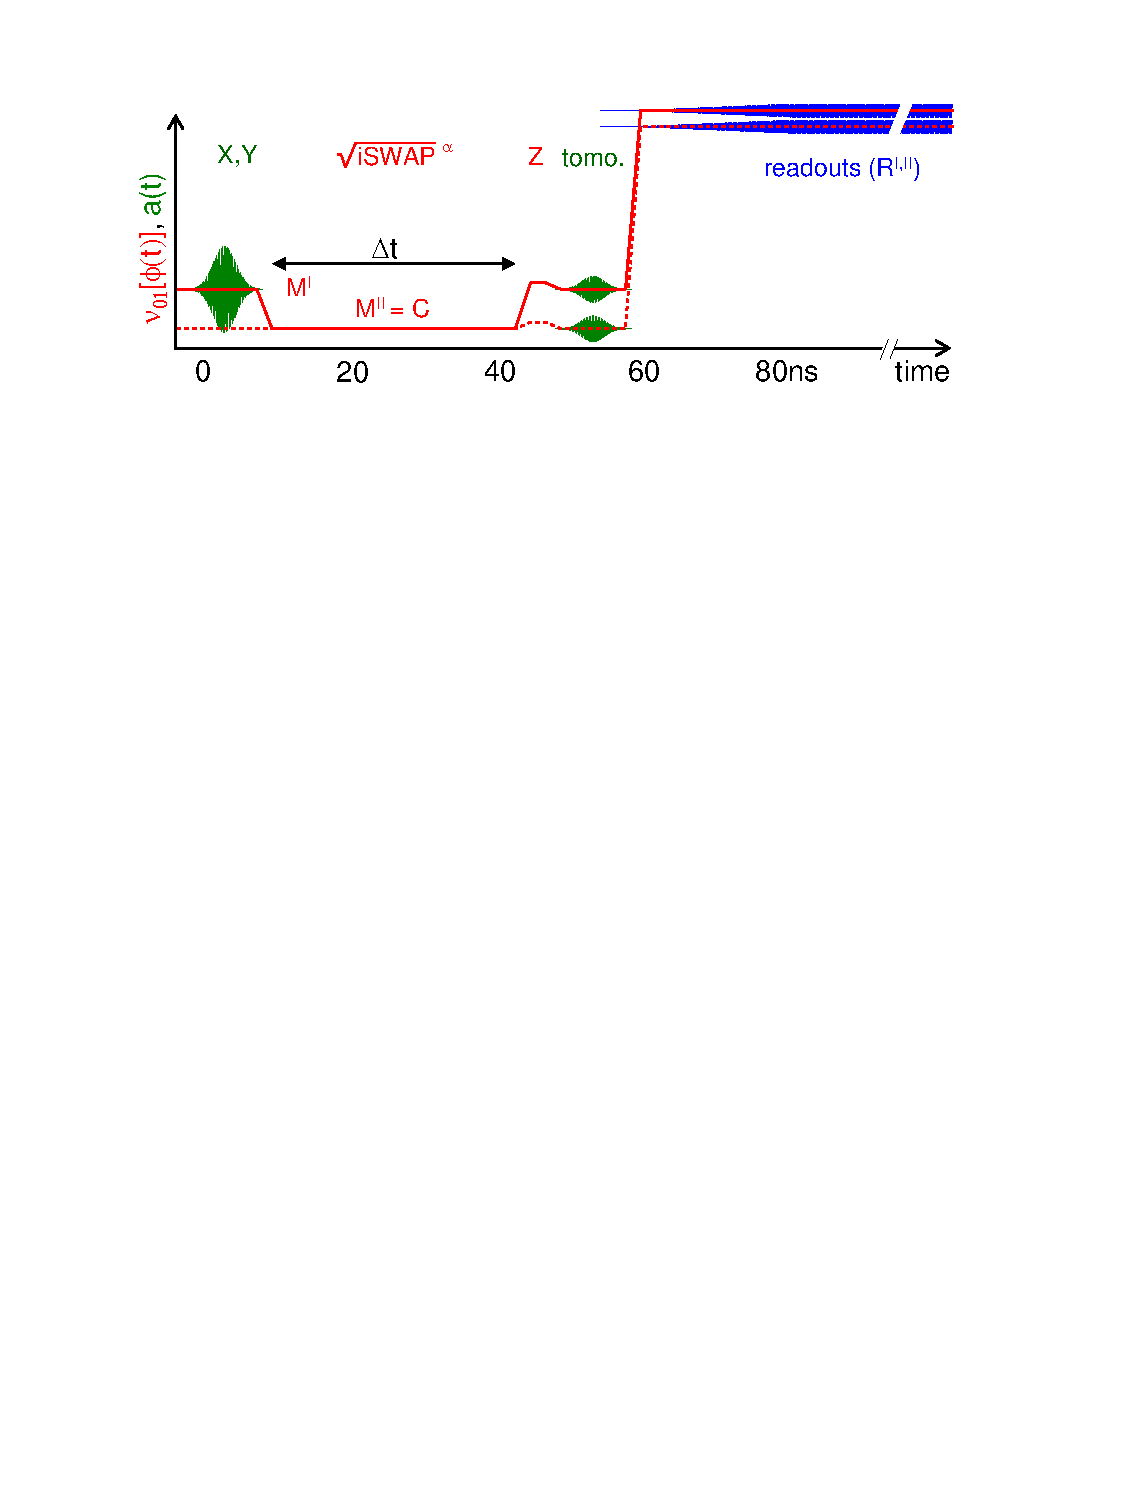
\includegraphics[width=0.8\textwidth]{./material/papers/iswap/figures/iswap_gate_pulse_sequence}
	\label{fig:ISwapPulseSequence}
	\caption{}
\end{figure}

\begin{figure}
  \flushright
	\includegraphics[width=1\textwidth]{"./data/ct5/2011_02_09 preparation of bell states/bell matrices"}
	\caption{Experimentially created $\ket{\psi_+}$ ($F = 0.91$) and $\ket{\psi_-}$ ($F=0.93$) states}
	\label{fig:BellStates}
\end{figure}

\subsection{Violation of the Bell Inequality}

\begin{figure}
	\centering
		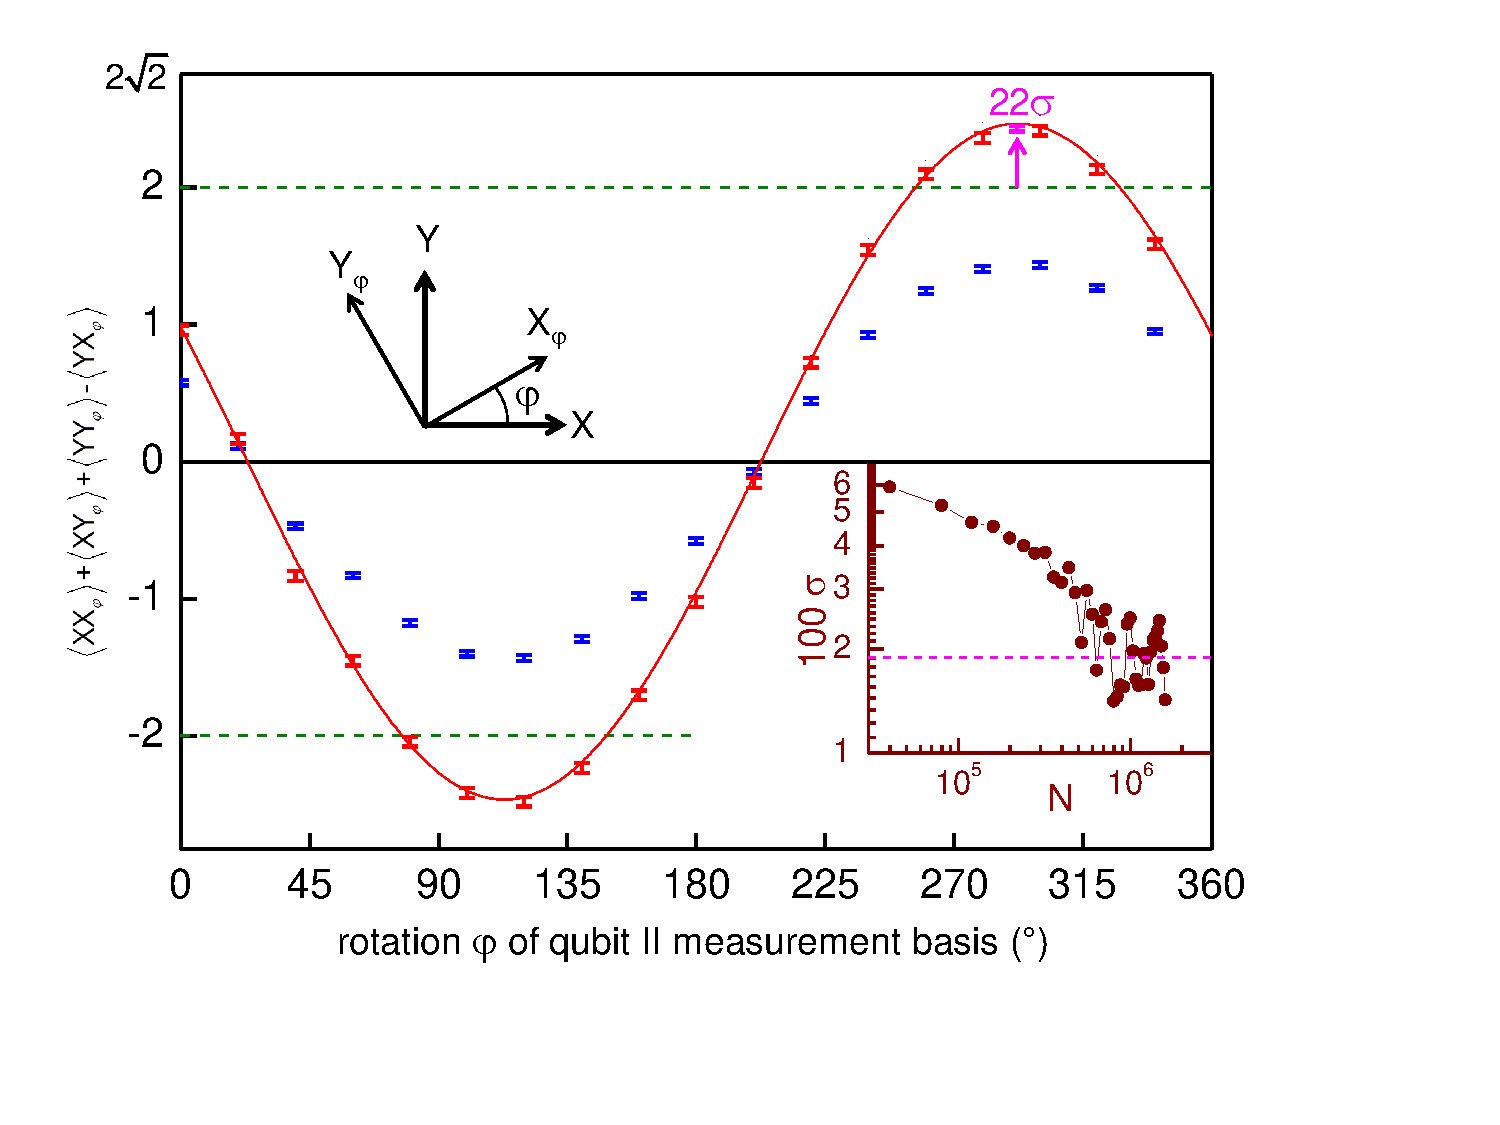
\includegraphics[width=0.8\textwidth]{./material/papers/iswap/figures/chsh}
	\label{fig:CHSH}
	\caption{}
\end{figure}

\begin{equation}
\mathrm{CHSH} = \mathrm{QS}+\mathrm{RS}+\mathrm{RT}-\mathrm{QT}
\end{equation}
with the operators $\mathrm{Q,R,S,T}$ being defined as

\begin{eqnarray}
	\begin{array}{cccccccc}
		\mathrm{Q} & = & \sigma_z^1 &&& \mathrm{S} & = & \sigma_z^2\cdot \cos{\phi}+\sigma_x^2 \cdot \sin{\phi} \\
		\mathrm{R} & = & \sigma_x^1 &&& \mathrm{T} & = & -\sigma_z^2\cdot \sin{\phi}+\sigma_x^2 \cdot \cos{\phi}
	\end{array}
\end{eqnarray} 

Here, the angle $\phi$ is a parameter that should be chosen in accordance to the phase of the Bell state on which it is applied.

\subsection{Quantum State Tomography of Two-Qubit States}

Quantum state tomography is the procedure of experimentally determining an unknown quantum state\citep{michael_a._nielsen_quantum_2000}.

The density matrix of an n-qubit system can be written in general form as
\begin{eqnarray}
\rho & = & \sum\limits_{v_1,v_2\hdots v_n} \frac{c_{v_1,v_2\hdots v_n} \sigma_{v_1}\otimes \sigma_{v_2}\hdots \sigma_{v_n}}{2^n} \label{eq:state_tomography_state_representation} \\
c_{v_1,v_2\hdots v_n} & = & \mathrm{tr}\left(\sigma_{v_1}\otimes \sigma_{v_2}\hdots \otimes\sigma_{v_n} \; \rho \right)  \label{eq:state_tomography_coefficients}
\end{eqnarray}
where $v_i \in \left\{ X,Y,Z,I\right\}$ and $n$ gives the number of qubits in the system and where the $c_{v_1,v_2\hdots v_n}$ are real-valued coefficients that fully describe the given density matrix. To reconstruct the density matrix of an experimental quantum system in a well-prepared state it is therefore sufficient to measure the expectation values of these $n^2-1$ coefficients on an ensemble of identically prepared systems. However, statistical and systematic measurement errors can yield a set of coefficients that corresponds to a {\it non-physical} density matrix which violates either the positivity or unity-trace requirement. In the following paragraph we will therefore discuss a technique with which one can estimate the density matrix of a system in a more correct way.

\subsubsection{Maximum Likelihood Estimation of Quantum States}

A method which is often used in quantum state tomography is the so-called {\it maximum-likelihood} technique. Rather than directly calculating the density matrix of the system from the obtained expectation values $c_{v_1,v_2\hdots v_n}$, it calculates the joint probability of measuring a set $\{c_{X,X,\hdots,X},c_{Y,X,\hdots,X},\hdots,c_{I,I,\hdots,I}\}$ for a given estimate of the density matrix $\hat{\rho}$. By numerically or analytically maximizing this joint probability over the set of possible density matrices we obtain the density matrix which is most likely to have produced the set of measurement outcomes that we have observed.

The joint measurement operators $\Sigma_j = \sigma_{v_1}\otimes \sigma_{v_2}\hdots \otimes\sigma_{v_n}$ have the eigenvalues $\pm 1$ and can thus be written as 
\begin{equation}
\sigma_{v_1}\otimes \sigma_{v_2}\hdots \otimes\sigma_{v_n} = \ket{+_j}\bra{+_j}-\ket{-_j}\bra{-_j}
\end{equation}
where $\ket{-_j}$ and $\ket{-_j}$ are the eigenstates corresponding to the eigenvalues $\pm 1$ of $\Sigma_j$. The expectation value $\langle \Sigma_j \rangle$ can be estimated by the quantity
\begin{equation}
\widehat{\langle \Sigma_j \rangle}_\rho = \frac{1}{l}\sum\limits_{i = 1}^l M_i(\Sigma_j,\rho) \label{eq:tomography_measurement_estimator}
\end{equation}
 where $M_i(M,\rho)$ denotes the outcome of the $i$-th measurement of the operator $M$ on the state described by the density matrix $\rho$. This quantity is binomially distributed with the expectation value $E(\widehat{\langle \Sigma_j \rangle}_\rho) = \langle \Sigma_j \rangle_\rho$ and the variance $\sigma^2(\widehat{\langle \Sigma_j \rangle}_\rho) = 1/l \cdot (1-\langle \Sigma_j \rangle_\rho^2)$. For large sample sizes $l$, the binomial distribution can be well approximated by a normal distribution with the same expectation value and variance. The joint probability of obtaining a set of measurement values $\{s_1,\hdots,s_{n^2-1}\}$ for the set of operators $\{\widehat{\langle\Sigma_1 \rangle}_\rho,\hdots,\widehat{\langle\Sigma_{n^2-1} \rangle}_\rho\}$ is then given as
\begin{equation}
P\left(\widehat{\langle \Sigma_1 \rangle }_\rho = s_1;\hdots;\widehat{\langle \Sigma_{n^2-1} \rangle}_\rho =  s_{n^2-1}\right) = \prod\limits_{i = 1}^{n^2-1} \exp{\left(-\frac{l}{2}\frac{(s_i-\langle \Sigma_i \rangle_\rho)^2}{1-\langle \Sigma_i \rangle_\rho^2}\right)}
\end{equation}
By maximizing this probability (or the logarithm of it) we obtain an estimate of the density matrix $\rho$ of the quantum state. This technique also allows us to include further optimization parameters when calculating the joint probability. This is useful for modeling e.g. systematic errors of the measurement or preparation process, which can be described by modifying the operators contained in the probability sum. A common source of errors in our tomography measurements are errors in the microwave pulses used to drive the qubit. Since our measurement apparatus permits us only to measure the $\sigma_z$ operator of each qubit we have to perform $\pi/2$ rotations about the $Y$ or $-X$ axes of the Bloch sphere of each individual qubit in order to measure the values of the $\sigma_x$ and $\sigma_y$ operators, which we therefore replace with an effective measurement of each qubits $\sigma_z$ operator preceded by a rotation $R_{\nu_i}$ given as
\begin{eqnarray}
R_{X} & = & \exp{\left( -i \sigma_y \pi / 4\right)} \\
R_{Y} & = & \exp{\left( +i \sigma_x \pi / 4\right)} 
\end{eqnarray}
Phase and amplitude errors can be modeled as
\begin{eqnarray}
R_{X} & = & \exp{\left( -i \left[+\sigma_y\cos{\alpha}+\sigma_x\sin{\alpha} \right] \left[\pi / 4+\gamma\right]\right)} \\
R_{Y} & = & \exp{\left( +i \left[-\sigma_y\sin{\beta}+\sigma_x\cos{\beta}\right] \left[\pi / 4+\delta\right]\right)} 
\end{eqnarray}
Here, $\alpha$ and $\beta$ represent phase errors whereas $\gamma$ and $\delta$ represent amplitude errors in the drive pulses.

\section{Realizing a Two-Qubit Gate}

\begin{figure}
   \centering
	 \includegraphics[width=1.\textwidth]{"./data/ct5/film of swap/pauli_set_vs_time_with_simulation"}
	 \caption[test]{Measured Pauli operators $\sigma_i \otimes \sigma_j$ with $i,j \in \{X,Y,Z,I\}$ as a function of the interaction time. Shown are the 6 single-qubit operators as well as the 9 two-qubit correlation operators. The dashed line represents a master-equation simulation of the experiment.}
	 \label{fig:swap_pauli_set_vs_time_with_simulation}
\end{figure}

\subsection{Principle}

\begin{figure}[p]
	\centering
		\includegraphics[width=1.0\textwidth]{"./data/ct5/2011_04_21 - grover and tomo/good_data/process -matrices 1"}
	\label{fig:ProcessInputOutputMatrices1}
	\caption{The input-output density matrix of the quantum process tomography of the $\sqrt{i\mathrm{SWAP}}$ gate. Shown are the measured density matrices of 16 different input states and the corresponding output matrices with their state fidelities. The ideal matrices are overlaid in red.}
\end{figure}

\begin{figure}[p]
	\centering
		\includegraphics[width=1\textwidth]{"./data/ct5/2011_04_21 - grover and tomo/good_data/process -matrices 2"}
	\label{fig:ProcessInputOutputMatrices2}
	\caption{The input-output density matrix of the quantum process tomography of the $\sqrt{i\mathrm{SWAP}}$ gate. Shown are the measured density matrices of 16 different input states and the corresponding output matrices with their state fidelities. The ideal matrices are overlaid in red.}
\end{figure}

\subsection{Experimental Implementation}

\subsection{Quantum Process Tomography of the Gate}

\subsubsection{Introduction \& Principle}

\subsubsection{Implementation}

A quantum process can be described as a map $\mathcal{E} : \rho_\mathcal{H} \to \rho_\mathcal{H}$ that maps a density matrix $\rho$ defined in a Hilbert space $Q_1$ to another density matrix $\mathcal{E}(\rho)$ defined in a target Hilbert space $Q_2$ and fulfilling three axiomatic properties \cite{michael_a._nielsen_quantum_2000,haroche_exploring_2006}:

\begin{axiom}
$\mathrm{tr}\left[\mathcal{E}(\rho)\right]$ is the probability that the process represented by $\mathcal{E}$ occurs, when $\rho$ is the initial state.
\end{axiom}

\begin{axiom}
$\mathcal{E}$ is a {\it convex-linear map} on the set of density matrices, that is, for probabilities $\left\{p_i\right\}$,

  \begin{equation}
	  \mathcal{E}\left(\sum\limits_i p_i \rho_i\right) = \sum\limits_i p_i \mathcal{E}(\rho_i)
	\end{equation}
\end{axiom}

\begin{axiom}
$\mathcal{E}$ is a {\it completely-positive} map. That is, if $\mathcal{E}$  maps density operators of system $Q_1$ to density operators of system $Q_2$, then $\mathcal{E}(A)$ must be positive for any positive operator $A$. Furthermore, if we introduce an extra system $R$ of arbitrary dimensionality, it must be true that $(\mathcal{I}\otimes \mathcal{E})(A)$ is positive for any positive operator $A$ on the combined system $RQ_1$, where $\mathcal{I}$ denotes the identity map on system $R$.
\end{axiom}
As shown in \cite{michael_a._nielsen_quantum_2000}, any quantum process fulfilling these criteria can be written in the form

\begin{equation}
  \mathcal{E}(\rho) = \sum\limits_i E_i \rho E_i^\dagger \label{eq:process_operator_sum_representation}
\end{equation}
for some set of operators $\{ E_i \}$ which map the input Hilbert space to the output Hilbert space, and $\sum_i E_i^\dagger E_i \le I$.

Now, if we express the operators $E_i$ in a different operator basis $\tilde{E}_j$ such that $E_i = \sum_j a_{ij} \tilde{E}_{j}$ and insert into eq. (\ref{eq:process_operator_sum_representation}), we obtain

\begin{eqnarray}
 \mathcal{E}(\rho) & = & \sum\limits_i \sum\limits_j a_{ij} \tilde{E}_j \;\rho\; \sum\limits_k a_{ik}^* \tilde{E}_k^\dagger \\
& = & \sum\limits_{j,k}\tilde{E}_j \; \rho \; \tilde{E}_k^\dagger \sum\limits_i a_{ij} a_{ik}^* \\
& = & \sum\limits_{j,k}\tilde{E}_j \; \rho \; \tilde{E}_k^\dagger \; \chi_{jk} \label{eq:process_chi_representation}
\end{eqnarray}
where we defined $\chi_{jk} = \sum\limits_i a_{ij} a_{ik}^*$. This is the so-called $\chi$-matrix representation of the quantum process. Here, all the information on the process is contained in the $\chi$ matrix, which controls the action of the process-independent operators $\tilde{E}_i$ on the initial density matrix $\rho$.

Now, the goal of {\it quantum process tomography} is to obtain the coefficients of the $\chi$-matrix -- or any other complete representation of the process -- from a set of experimentally measured density matrices $\rho$ and $\mathcal{E}(\rho)$.

To achieve this, several techniques have been developed. The technique used in this work is the so-called {\it standard quantum process tomography (SQPT)}. This technique proceeds as follows:

\begin{enumerate}
\item Choose a set of operators $E_i$ that forms a full basis of $\mathcal{M}: Q_1 \to Q_2$. For n-qubit process tomography we usually choose $E_{i_1,i_2 \hdots i_n} = \sigma_{i_1}\otimes \sigma_{i_2}\hdots\otimes\sigma_{i_n}$, where $\sigma_i$ are the single-qubit Pauli operators and $i\in\{I,X,Y,Z\}$. 
\item Choose a set of pure quantum states $\ket{\phi_i}$ such that $\ket{\phi_i}\bra{\phi_i}$ span the whole space of input density matrices $\rho$. Usually, for a n-qubit system we choose $\phi = \{\ket{0},\ket{1},(\ket{0}+\ket{1})/\sqrt{2},(\ket{0}+i\ket{1})/\sqrt{2}\}^{\otimes n}$, where $^{\otimes n}$ denotes the n-dimensional Kronecker product of all possible permutations.
\item For each of the $\ket{\phi_i}$, determine $\mathcal{E}(\ket{\phi_i}\bra{\phi_i})$ by quantum state tomography. Usually we also determine $\ket{\phi_i}\bra{\phi_i}$ experimentally since the preparation of this state already entails small preparation errors that should be taken into account when performing quantum process tomography. 
\end{enumerate}

After having obtained the $\rho_i$ and $\mathcal{E}(\rho_i)$ one obtains the $\chi$-matrix by writing $\mathcal{E}(\rho_i) = \sum_j \lambda_{ij} \tilde{\rho}_j$, with some arbitrary basis $\tilde{\rho}_j$ and
letting $\tilde{E}_m \tilde{\rho}_j \tilde{E}_n^\dagger = \sum_k \beta_{jk}^{mn}\tilde{\rho}_k$. We can then insert into eq. (\ref{eq:process_chi_representation}) and obtain
\begin{eqnarray}
\sum\limits_k \lambda_{ik} \tilde{\rho}_k & = & \sum\limits_{m,n} \chi_{mn} \sum\limits_k \beta_{ik}^{mn} \tilde{\rho}_k  
\end{eqnarray}
This directly yields $\lambda_{ik} = \sum_{m,n}\beta_{ik}^{mn}\; \chi_{mn}$, which, by linear inversion,  gives $\chi$.

\subsubsection{The Kraus Representation of the Quantum Process}

Besides the $\chi$-matrix representation, there is another useful way of expressing a quantum map, the so called {\it Kraus representation}, which is given as

\begin{equation}
 \mathcal{E}(\rho) = \sum\limits_i M_i \; \rho \; M_i^\dagger \label{eq:process_kraus_representation}
\end{equation}

It can be shown \citep{haroche_exploring_2006} that this sum contains at most $N$ elements, where $N$ is the dimension of the Hilbert space of the density matrix $\rho$. We can go from the $\chi$ representation to the Kraus representation by changing the basis $\tilde{E}_i$ such that

\begin{equation}
	\tilde{E}_i = \sum\limits_l a_{il}\; \breve{E}_l
\end{equation}

which, for eq. (\ref{eq:process_chi_representation}), yields

\begin{eqnarray}
 \mathcal{E}(\rho) & = & \sum\limits_{j,k} \sum\limits_l a_{jl} \breve{E}_l \; \rho \sum\limits_m a_{km}^* \breve{E}_m^\dagger \; \chi_{jk} \\
 & = & \sum\limits_{l,m}  \breve{E}_l \; \rho \; \breve{E}_m^\dagger \; \sum\limits_{j,k} a_{jl} a_{km}^* \chi_{jk} \label{eq:process_chi_transformed}
\end{eqnarray}

The last sum on the right side of eq. (\ref{eq:process_chi_transformed}) corresponds to a change of coordinates of the matrix $\chi$. Now, we can pick the $a$ such that $\chi$ is diagonal in the new basis $\breve{E}$ and obtain

\begin{eqnarray}
 \mathcal{E}(\rho) & = &  \sum\limits_{l} \lambda_l \breve{E}_l \; \rho \; \breve{E}_l^\dagger \\
& = &  \sum\limits_{l} M_l \; \rho \; M_l^\dagger
\end{eqnarray}
with $\lambda_l$ being the $l$-th eigenvalue of the $\chi$ matrix with the eigen-operator $\breve{E}_l$ and $M_{l} = \sqrt{\lambda_l} \breve{E}_l$.

\subsection{Gate Fidelity}

\subsection{Gate Error Analysis}

Tomographic errors are removed from the process map of our $\sqrt{iSWAP}$
gate using the following method. The measured Pauli sets corresponding
to the sixteen input states are first fitted by a model including
errors both in the preparation of the state (index $prep$) and in
the tomographic pulses (index $tomo$). The errors included are angular
errors $\varepsilon_{\mathrm{I,II}}^{\mathrm{prep}}$ on the nominal
$\pi$ rotations around $X_{\mathrm{I,II}}$, $\eta_{\mathrm{I,II}}^{\mathrm{prep,tomo}}$and
$\delta_{\mathrm{I,II}}^{\mathrm{prep,tomo}}$ on the nominal $\pi/2$
rotations around $X_{\mathrm{I,II}}$ and $Y_{\mathrm{I,II}}$, a
possible departure $\xi_{\mathrm{I,II}}$ from orthogonality of $\left(\overrightarrow{X_{\mathrm{I}}},\overrightarrow{Y_{\mathrm{I}}}\right)$
and $\left(\overrightarrow{X_{\mathrm{II}}},\overrightarrow{Y_{\mathrm{II}}}\right)$,
and a possible rotation $\mu_{\mathrm{I,II}}$ of the tomographic
$XY$ frame with respect to the preparation one. The rotation operators
used for preparing the states and doing their tomography are thus
given by

\[
\begin{array}{c}
X_{\mathrm{I,II}}^{\mathrm{prep}}(\pi)=e^{-\mathrm{i}\left(\pi+\varepsilon_{\mathrm{I,II}}^{\mathrm{prep}}\right)\sigma_{\mathrm{x}}^{\mathrm{I,II}}/2},\\
X_{\mathrm{I,II}}^{\mathrm{prep}}(-\pi/2)=e^{+\mathrm{i}\left(\pi/2+\eta_{\mathrm{I,II}}^{\mathrm{prep}}\right)\sigma_{\mathrm{x}}^{\mathrm{I,II}}/2},\\
Y_{\mathrm{I,II}}^{\mathrm{prep}}(\pi/2)=e^{-\mathrm{i}\left(\pi/2+\delta_{\mathrm{I,II}}^{\mathrm{prep}}\right)\left[\mathrm{cos}\left(\xi_{\mathrm{I,II}}\right)\sigma_{\mathrm{y}}^{\mathrm{I,II}}\mathrm{-sin}\left(\xi_{\mathrm{I,II}}\right)\sigma_{\mathrm{x}}^{\mathrm{I,II}}\right]/2},\\
X_{\mathrm{I,II}}^{\mathrm{tomo}}(\pi/2)=e^{-\mathrm{i}\left(\pi/2+\eta_{\mathrm{I,II}}^{\mathrm{tomo}}\right)\left[\mathrm{\mathrm{sin}\left(\mu_{I,II}\right)\sigma_{x}^{I,II}+cos}\left(\mu_{\mathrm{I,II}}\right)\sigma_{\mathrm{y}}^{\mathrm{I,II}}\right]/2},\\
Y_{\mathrm{I,II}}^{\mathrm{tomo}}(-\pi/2)=e^{+\mathrm{i}\left(\pi/2+\delta_{\mathrm{I,II}}^{\mathrm{tomo}}\right)\left[\mathrm{cos}\left(\mu_{\mathrm{I,II}}+\xi_{\mathrm{I,II}}\right)\sigma_{\mathrm{y}}^{\mathrm{I,II}}\mathrm{-sin}\left(\mu_{\mathrm{I,II}}+\xi_{\mathrm{I,II}}\right)\sigma_{x}^{\mathrm{I,II}}\right]/2}.\end{array}\]
The sixteen input states are then $\left\{ \rho_{\mathrm{in}}^{\mathrm{e}}=U\left|0\right\rangle \left\langle 0\right|U^{\dagger}\right\} $
with $\left\{ U\right\} =\{I_{\mathrm{I}},X_{\mathrm{I}}^{\mathrm{prep}}(\pi),Y_{\mathrm{I}}^{\mathrm{prep}}(\pi/2),X_{\mathrm{I}}^{\mathrm{prep}}(-\pi/2)\}\otimes\{I_{\mathrm{II}},X_{\mathrm{II}}^{\mathrm{prep}}(\pi),Y_{\mathrm{II}}^{\mathrm{prep}}(\pi/2),X_{\mathrm{II}}^{\mathrm{prep}}(-\pi/2)\}$,
and each input state yields a Pauli set $\left\{ \left\langle P_{\mathrm{k}}^{\mathrm{e}}\right\rangle =Tr\left(\rho_{\mathrm{in}}^{\mathrm{e}}P_{\mathrm{k}}^{\mathrm{e}}\right)\right\} $
with $\left\{ P_{\mathrm{k}}^{\mathrm{e}}\right\} =\{I_{\mathrm{I}},X_{\mathrm{I}}^{\mathrm{e}},Y_{\mathrm{I}}^{\mathrm{e}},Z_{\mathrm{I}}\}\otimes\{I_{\mathrm{II}},X_{\mathrm{II}}^{\mathrm{e}},Y_{\mathrm{II}}^{\mathrm{e}},Z_{\mathrm{II}}\}$,
$X^{\mathrm{e}}=Y^{\mathrm{tomo}}(-\pi/2)^{\dagger}\sigma_{z}Y^{\mathrm{tomo}}(-\pi/2)$,
and $Y^{\mathrm{e}}=X^{\mathrm{tomo}}(\pi/2)^{\dagger}\sigma_{\mathrm{z}}X^{\mathrm{tomo}}(\pi/2)$.
Figure S5.1 shows the best fit of the modelled $\left\{ \left\langle P_{k}^{e}\right\rangle \right\} $
set to the measured input Pauli sets, yielding $\varepsilon_{\mathrm{I}}^{\mathrm{prep}}=-1\text{\textdegree}$,
$\varepsilon_{\mathrm{II}}^{\mathrm{prep}}=-3\text{\textdegree}$,
$\eta_{\mathrm{I}}^{\mathrm{prep}}=3\text{\textdegree}$, $\mathrm{\eta}_{\mathrm{II}}^{\mathrm{prep}}=4\text{\textdegree}$,
$\delta_{\mathrm{I}}^{\mathrm{prep}}=-6\text{\textdegree}$, $\delta_{\mathrm{II}}^{\mathrm{prep}}=-3\text{\textdegree}$,
$\eta_{\mathrm{I}}^{\mathrm{tomo}}=-6\text{\textdegree}$, $\eta_{\mathrm{II}}^{\mathrm{tomo}}=-4\text{\textdegree}$,
$\lambda_{\mathrm{I}}^{t\mathrm{omo}}=12\text{\textdegree}$, $\lambda_{\mathrm{II}}^{\mathrm{tomo}}=5\text{\textdegree}$,
$\xi_{\mathrm{I}}=1\text{\textdegree}$, $\xi_{\mathrm{II}}=-2\text{\textdegree}$,
and $\mu_{\mathrm{I}}=\mu_{\mathrm{II}}=-11\text{\textdegree}$.

Knowing the tomographic errors and thus $\left\{ \left\langle P_{\mathrm{k}}^{\mathrm{e}}\right\rangle \right\} $,
we then invert the linear relation $\left\{ \left\langle P_{\mathrm{k}}^{\mathrm{e}}\right\rangle =Tr\left(\rho P_{\mathrm{k}}^{\mathrm{e}}\right)\right\} $
to find the $16\times16$ matrix $B$ that links the vector $\overrightarrow{\left\langle P_{\mathrm{k}}^{\mathrm{e}}\right\rangle }$
to the columnized density matrix $\overrightarrow{\rho}$, i.e. $\overrightarrow{\rho}=B.\overrightarrow{\left\langle P_{\mathrm{k}}^{\mathrm{e}}\right\rangle }$.
The matrix $B$ is finally applied to the measured sixteen input and
sixteen output Pauli sets to find the sixteen $(\rho_{\mathrm{in},},\rho_{\mathrm{out}})_{\mathrm{k}}$
couples to be used for calculating the gate map.


%-Discuss the realization of a 2 qubit gate:
%  -Principle
%  -Implementation & Pulse Sequency
%  -Characterization through Quantum Process Tomography:
%     -Principles: State tomography, Pauli set, process tomography
%     -Discuss alternative representations of the process information:
%        -Chi matrix, Choi matrix, S, log S, Kraus operator representation
%  		-Errors: Discuss simulations, error models and possible reasons for discrepancies

\begin{figure}
	\centering
		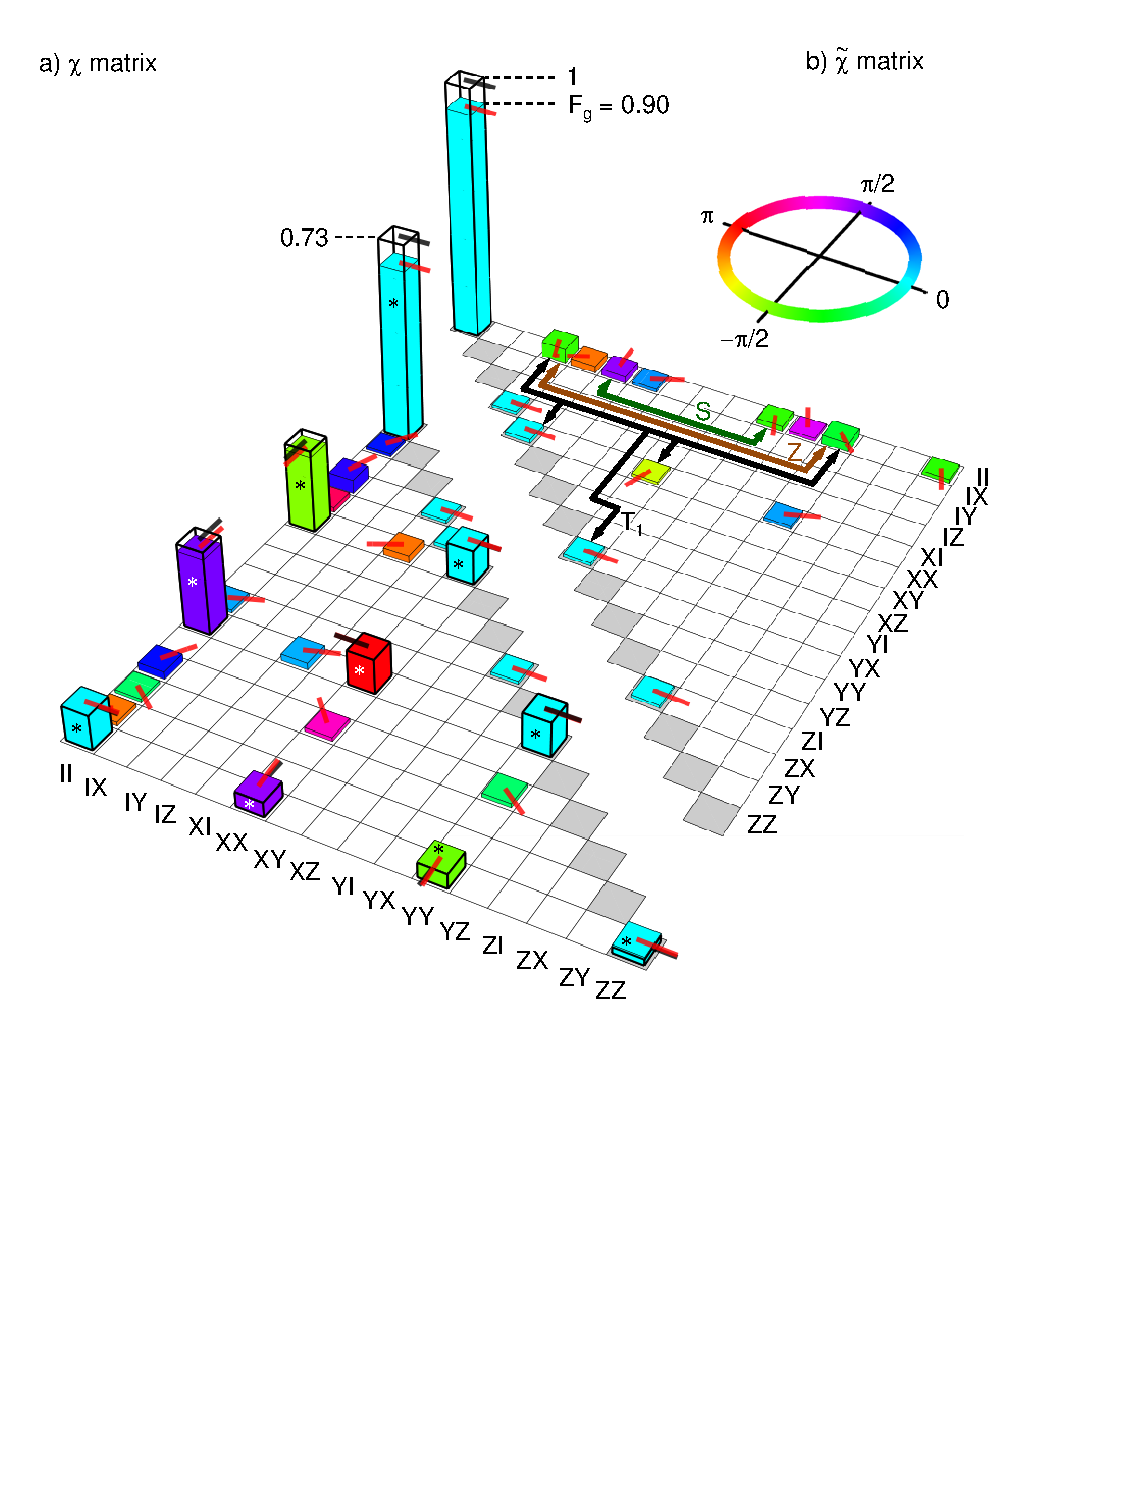
\includegraphics[width=1.\textwidth]{./material/papers/iswap/figures/chi_matrix_and_error_process}
	\label{fig:GateChiMatrixAndErrorProcess}
	\caption{}
\end{figure}


\chapter{Running the Grover Search Algorithm}

This chapter will describe the experimental implementation of the so-called {\it Grover search algorithm} with our two-qubit quantum processor. The first section will provide a short introduction of the algorithm and motivate the interest in realizing it. The following sections will then discuss the details of the experimental realization of this algorithm. We will discuss the results that we obtained and compare the algorithm fidelity and runtime to that of an equivalent, classical algorithm. Finally, we will analyze all relevant errors made in our experiment.

\section{Introduction \& Motivation}

Search algorithms are of great importance in many domains of mathematics and computer science. One such search problem that often arises and which will be discussed in the following sections can be formulated in simple terms as follows:

\begin{theorem}
Assume that we have a search space $\begin{mathcal}S\end{mathcal}$ that consists of a finite number $N$ of states $s \in \begin{mathcal}S\end{mathcal}$. The solution to our search problem corresponds to a finite subset of $M$ states of the search space $\begin{mathcal}T\end{mathcal} \subset \begin{mathcal}S\end{mathcal}$. We can then define a search function $\Or(s):\begin{mathcal}S\end{mathcal}\to \{0,1\}$ that discriminates between states that solve the search problem and states that don't, such that $\Or(s) = 1$ for $s \in \begin{mathcal}T\end{mathcal}$ and $\Or(s) = 0$ otherwise.
\end{theorem}

Using this definition of the search problem, the goal of a search algorithm is to find all states $t\in\begin{mathcal}S\end{mathcal}$ for which $\Or(t) = 1$. In the following sections, for the sake of simplicity we will assume in the following sections that the solution set $\begin{mathcal}T\end{mathcal}$ contains only one single state $t$. This special case can easily be generalized to cases where more than one solution exists to the search problem.

\smallskip

The first step in order to solve a search problem of the kind described above is to map the problem above to a form suitable for solution by a digital (quantum) computer. For this, we first number and encode the $N$ input states $s_i \in \begin{mathcal}S\end{mathcal}$ in binary form such that $s_i = \sum\limits_{j=0}^l s_{ij}2^j $, where $l$ is the minimum required length of a binary register that can hold all $N$ input states. With this definition, it is then also trivial to reformulate $\Or$ such that the function operates on a binary input register instead of the original input states. 

\smallskip

Using these assumptions and definitions, it can then be shown that the most efficient classical search algorithm for solving the search problem above will use $\begin{mathcal}O\end{mathcal}(N)$ calls of the function $\Or$ to find the solution $t$ of the search problem. Assuming that the time to evaluate the function $\Or$ is far superior to the time needed to perform any other operation during the search algorithm, the number of calls to $\Or$ also corresponds approximately to the runtime of the whole search algorithm.

\smallskip

Amazingly, in 1997, \cite{Grover_Quantum_1997} found a quantum algorithm that could solve exactly the same search problem with only $\begin{mathcal}O\end{mathcal}(\sqrt{N})$ calls to the function $\Or$. His algorithm achieves this by repeatedly calling a quantum-mechanical implementation of the function $\Or$ with a highly superposed qubit state and applying a special operator to the output state afterwards. The individual steps of the algorithm are straightforward and are given as follows:

\begin{enumerate}
 \item Initialize a qubit register to the state $\ket{\psi} = \ket{0}$ (corresponding to a binary input state $\ket{0000\hdots0_B}$)
 \item Apply the generalized Hadamard operation to the qubit register, producing a fully superposed quantum state $$\ket{\psi} = \frac{1}{\sqrt{N}}\sum\limits_{i=0}^{N-1} \ket{i}$$
 \item Repeat the following sequence $\begin{mathcal}O\end{mathcal}(\sqrt{N})$ times:
 \subitem a) Apply the {\it Oracle operator} $\ket{i}\to (-1)^{\Or(i)}\ket{i}$ to the state $\ket{\psi}$
 \subitem b) Apply the {\it diffusion operator} $\ket{i} \to -\ket{i}+\frac{2}{N}\sum\limits_{i=0}^{N-1}\ket{j}$ to the state $\ket{\psi}$
	\item Measure the state of the quantum register
\end{enumerate}

Here, we have numerated the states of the qubit register from $\ket{0}$ to $\ket{N-1}$. The algorithm makes use of quantum parallelism to solve the search problem $\begin{mathcal}O\end{mathcal}(\sqrt{N})$ times faster than the most efficient classical algorithm. To understand better the action of the algorithm, the different steps of the Grover algorithm can be rephrased in the following, more intuitive way:

\begin{itemize}
\item First, it creates a fully superposed quantum state which contains all possible solutions to the search problem at once. The amplitudes and phases of each individual state are all equal in the beginning.
\item Then, it applies the so-called Oracle operator to this superposed state. The effect of the Oracle is to flip the sign of the states $t$ that corresponds to a solution of the search problem, i.e. for which $\Or(t)=1$. As will be shown later, such an Oracle operator can be implemented in a straightforward way for any possible classical search function.
\item In the next step, it applies a diffusion operator to the quantum state which transfers a fraction of the amplitude of all states with positive amplitude to the states with negative amplitude, increasing the amplitude of the latter in expense of the amplitude of the former. In this process, all states whose amplitude signs have been flipped get reset to positive values.
\item Repeating these two operations increases the amplitude of the states which correspond to a solution of the search problem in a monotonous way until the amplitudes of all the other states are zero. When all the amplitude has been transferred to those states, the process reverses and the amplitude is transferred back to the other states. Hence it is crucial to stop the repeated application of the Oracle and diffusion operators after the right number of iterations.
\end{itemize}

As can be seen, the Grover algorithm uses quantum superposition as a resource to ``crawl'' a given search space faster than any possible classical algorithm, therefore speeding up the finding of a solution to the search problem. However, the crux of the algorithm is the way in which it extracts the knowledge of the search space it acquires when calling the search function with a superposed quantum state. This is very important since when applying the search function to a superposed quantum state the resulting output state will indeed contain the values of the search function for all possible values, but it is usually impossible to extract the full information from this state with one single measurement since any measurement performed on the qubit state will project it to an eigenstate of the measurement operator, thus destroying most of the information contained in the state. It would be possible to obtain the full information on the resulting quantum state by performing quantum state tomography, however for a $N$ qubit register this would involve $2^N$ preparation and measurement cycles, thereby destroying any potential quantum-speed. It is therefore necessary to find a method by which one can extract the knowledge on the search function encoded in the quantum state in less than $\begin{mathcal}O\end{mathcal}(N)$ operations. This is exactly what the diffusion operator $D$ achieves by converting the phase information contained in a superposition state to which the Oracle operator has been applied to a gain in amplitude of all states with negative amplitudes.

\subsection{Deriving the Grover Algorithm from Schrödinger's Equation}

\begin{floatingfigure}[r]{5.5cm}
\includegraphics[width=5.2cm]{"./material/papers/grover/grover_derivation_schroedinger"}
\caption{A wavefunction $\psi(x)$ and potential $V(x)$ defined on a grid of points $x_1,\hdots,x_N$.}
\label{fig:GroverDerivationSchroedinger}
\end{floatingfigure}

An interesting derivation of this algorithm starting from Schrödinger's equation has been given in a seminal paper by \cite{grover_schrodingers_2001} and shall be briefly rediscussed here. The derivation begins by considering a quantum system governed by Schrödinger's equation, which can be written as (omitting all physical constants for the sake of clarity)

\begin{equation}
-i\frac{\delta}{\delta t}\psi(x,t) = \frac{\delta^2}{\delta x^2}\psi(x,t)-V(x)\psi(x,t) \label{eq:grover_derivation}
\end{equation}

Here $\psi(x,t)$ describes the wave-function and $V$ is a time-indepenent potential. Let us assume that the potential $V(x)$ is shaped as in fig. \ref{fig:GroverDerivationSchroedinger}, i.e. possessing a local minimum of energy. When one initializes the system to a state $\psi_0(x,t_0)$ and lets it evolve for a given time, the resulting state $\psi(x,t)$ will have a tendency to have a high probability density in the local minimum of the potential, thus ``falling'' into the potential minimum much like a classical system would.

It is thus interesting to ask if one could encode the solution to some hard problem as a point of minimum energy $x_0$ of a potential $V(x)$ and design an algorithm that would take an initial state $\psi_0(x,t_0)$ and let it evolve into a state that has a high probability around $x_0$. Most problems in classical computer science involve functions operating on binary numbers of fixed length, so to encode these numbers we can discretize our wavefunction $\psi(x,t)$ using a regular grid of points $x_i$ with a spacing $dx$, as shown in fig. \ref{fig:GroverDerivationSchroedinger}b. When we discretize the time evolution of eq. \ref{eq:grover_derivation} in steps $dt$ as well and define $\epsilon = dt/dx^2$, we obtain a new equation of the form

\begin{equation}
-\frac{\psi_i^{t+dt}-\psi_x^{t}}{dt} = \frac{\psi_{i+1}^t+\psi_{i-1}^t-2\psi_x^t}{dx^2} -V(x_i)\psi_i^t
\end{equation}

where we have written $\psi(x_i,t)=\psi_i^t$. This equation can be written in matrix form as

\begin{equation}
\vec{\psi}^{t+dt} = S^t  \cdot \vec{\psi}^t
\end{equation}

with $S$ being a state transition matrix of the form

\begin{equation}
S = \left(
	\begin{array}{ccccc}
		1-2i\epsilon-iV(x_1)dt & i\epsilon & 0 & \hdots &  i\epsilon \\
		i \epsilon & 1-2i\epsilon -iV(x_2)dt & i\epsilon & \hdots & 0 \\
		0 & i\epsilon & \ddots & & \vdots \\
		\vdots & & & \ddots  & \vdots \\
		i \epsilon & 0 & \hdots & i\epsilon & 1 - 2i\epsilon -iV(x_n)dt
	\end{array}
 \right) \label{eq:grover_iteration_matrix}
\end{equation}

where we have used cyclic boundary conditions and defined $\epsilon = dt/dx^2$. To calculate the wavefunction at a finite evolution time we make use the Lie-Trotter formula

\begin{equation}
\exp{\left(A+B\right)} = \lim\limits_{N\to\infty}\left(\exp{\left(A/N\right)}\exp{\left(B/N\right)}\right)^N
\end{equation}

to write $\exp{\left(S\right)} \approx D\cdot R$ with 

\begin{eqnarray}
D & = & \left( 
		\begin{array}{cccccc}
		1-2i \epsilon & i\epsilon & 0 & 0 & \hdots & i\epsilon \\
		i \epsilon & 1 - 2i \epsilon & i \epsilon & 0 & \hdots & 0 \\
		\hdots & \ddots & & & & \vdots \\
		i \epsilon & 0 & 0 &  \hdots & i\epsilon & 1-2i \epsilon \\
		\end{array}
	\right)
\end{eqnarray}
and 
\begin{eqnarray}
R & = & \left( \begin{array}{ccccc}
	e^{-i V(x_1) dt} & 0 & \hdots & 0 \\
	0 & e^{-i V (x_2) dt} & \hdots & 0 \\
	0 & \hdots & & 0 & e^{-i V (x_N) dt} \\
	\end{array}
	\right)
\end{eqnarray}

This approximation is correct to $\begin{mathcal}O\end{mathcal}(\epsilon)$ up to an unrelevant renormalization factor. The technique of splitting up the full evolution operator into a product of two or more non-commuting evolution operators that are applied successively is widely used in digital quantum simulation \citep{lloyd_universal_1996,lanyon_universal_2011}. We can now repeatedly apply the matrix product $D\cdot R$ to the waveunction to obtain its state after a given finite time $\Delta t$ by writing

\begin{equation}
\vec{\psi}^{t+\Delta t} = \left(\prod\limits_{i = 1}^{\Delta t/dt} D\cdot R\right)\cdot \vec{\psi}^{t}
\end{equation}

As can be seen, the evolution of the wavefunction is governed by two processes: The interaction of the wavefunction with the potential $V$ and a diffusion process which mixes different spatial parts of the wavefunction. The operator $D$ resembles a Markov diffusion process since each row and column of the matrix sums up to unity, whereas $R$ changes the phase of each element of the wavefunction in accordance with the local potential seen by it. If we apply $R$ to a fully superposed initial state of the form $\psi_i = 1$ (we omit the normalization factor for clarity) and assume that $V_i = 0$ for $i \ne j$ and $V_j dt = \pi/2$, the element $\psi_j$ will get turned according to $\psi_j \to i\psi_j $, whereas all other elements $\psi_i$ will remain unchanged. Applying the operator $D$ to the resulting state will transform $\psi_j$ according to $\psi_j \to \psi_j(i+2\epsilon(1+i))$ with a corresponding amplitude $\sqrt{1+4\epsilon+\begin{mathcal}O\end{mathcal}(\epsilon^2)}$ and the adjacent states $\psi_{j\pm 1}$ according to $\psi_{j\pm 1} \to \psi_{j\pm 1}(1-\epsilon(1+i))$ with an amplitude $\sqrt{1-2\epsilon +\begin{mathcal}O\end{mathcal}(\epsilon^2)}$. Hence there is a transfer of amplitude between the state whose phase has been turned and its neighboring states. If we reset the phases of all the $\psi_i$ to zero afterwards, we can iterate the application of $D\cdot R$ until all of the amplitude has been transferred to the element $\psi_j$. This, in essence, is exactly what the Grover algorithm does with the only difference the matrix $D$ gets replaced with an unitary matrix

\begin{equation}
D = \left( \begin{array}{ccccc}
	-1+2/N & 2/N & 2/N & \hdots & 2/N \\
	2/N & -1 + 2/N & 2/N & \hdots & 2/N \\
	\vdots & & \ddots &  & \vdots \\
	2/N & 2/N & 2/N & \hdots & -1 + 2/N \\ 
	\end{array} \right) \label{eq:GroverDiffusionOperator}
\end{equation}

and $R$ with an unitary matrix 
\begin{eqnarray}
R & = & \mathrm{I}^{N\otimes N}-2\sum\limits_{i}\Or(i)\ket{i}\bra{i} \label{eq:GroverOracleFunction}
\end{eqnarray}
that implements the quantum Oracle operator for the search function $\Or$. These matrices are chosen such that the transfer of amplitude between the marked state and the others is maximized in each step of the algorithm . By repeating the $D\cdot R$ sequence $\begin{mathcal}O\end{mathcal}(\sqrt{N})$ times with these modified matrices, all the amplitude can be transferred to the basis state $\ket{j}$ for which $\Or(j)=1$, hence solving the search problem.

\subsection{Ancilla-based Implementation of the Algorithm}

\begin{figure}[ht!]
	\centering
		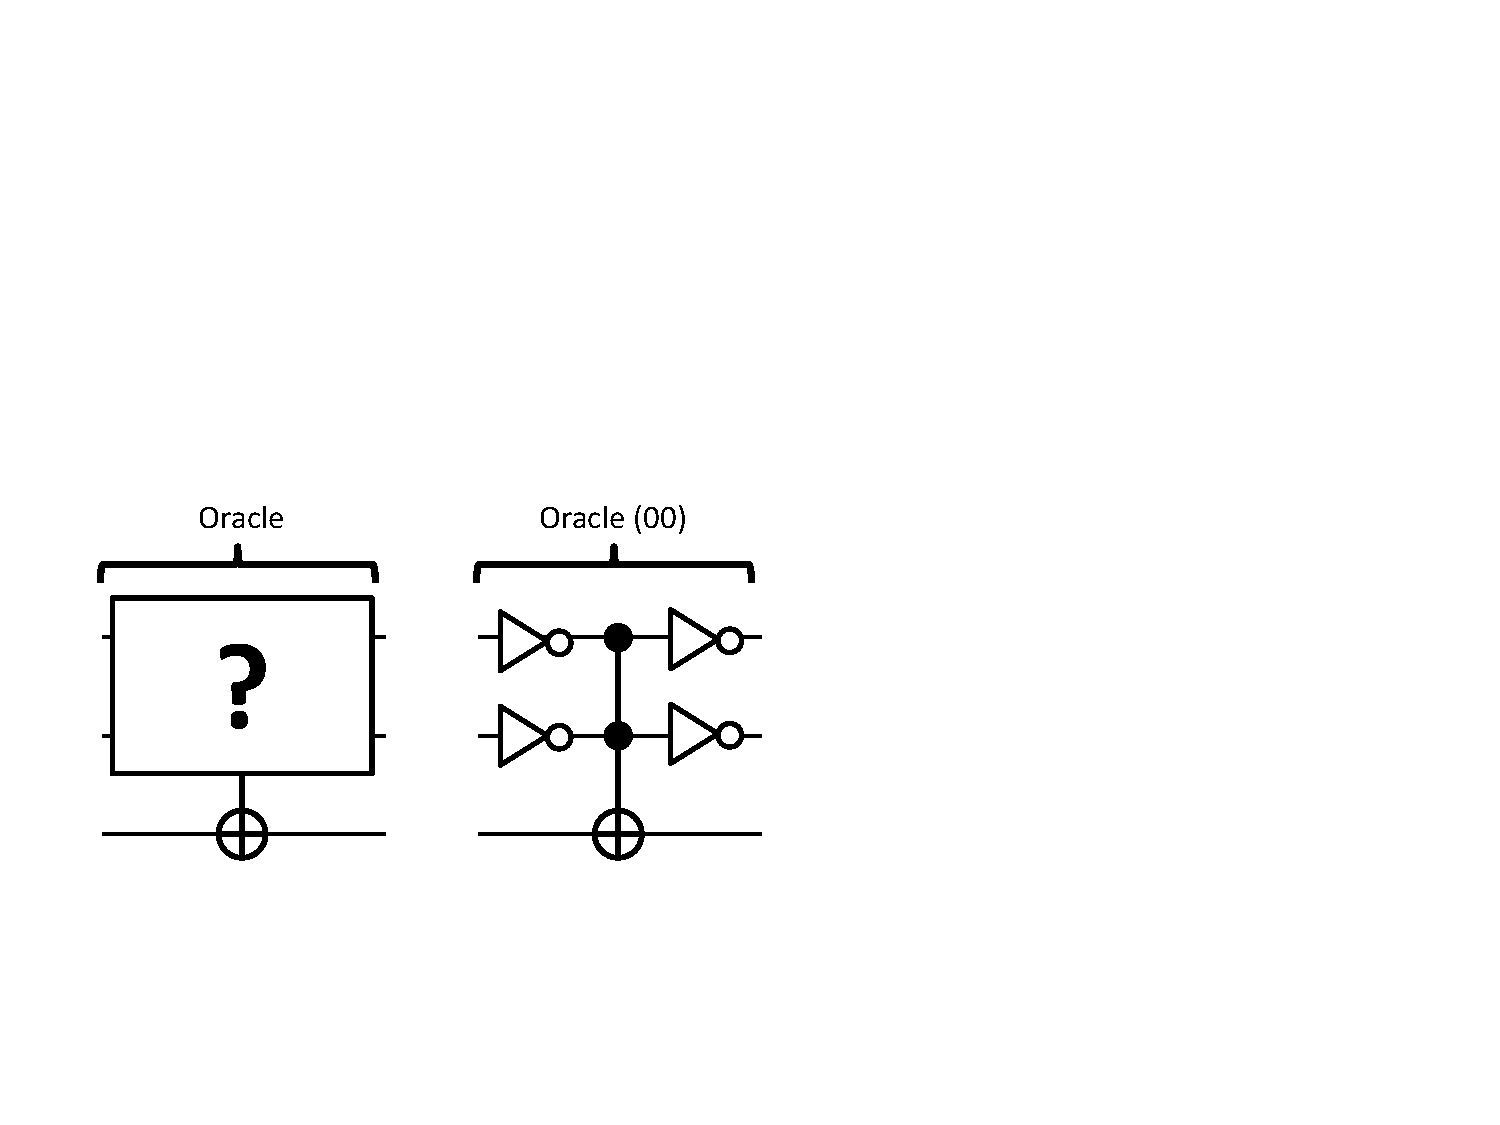
\includegraphics[width=1\textwidth]{./material/papers/grover/different_oracle_implementations}
	\caption[Implementations of the four possible Oracle functions used in the Grover search algorithm, using only reversible gate operations]{Implementations of the four possible Oracle functions used in the Grover search algorithm, using only reversible gate operations.}
	\label{fig:GroverOracleImplementations}
\end{figure}

The implementation of the Grover search algorithm outlined above encodes the value of the search function $\Or$ in the phase of the input state supplied to this function. This makes it hard to compare the algorithm to a classical search algorithm which operates on a binary input states and, in general, cannot encode the result of the search function directly in the input state. It is therefore useful to formulate a version of the Grover algorithm where the Oracle function does not directly encode the marked state in the input qubit register but uses an ancialla qubit to store the result of calling $\Or$. Such a representation of the algorithm is very useful since it can be directly compared to a classical algorithm implemented with reversible logic gates, thus making it possible to benchmark our algorithm against a classical counterpart. Exemplary implementations of ancilla-based search functions $\Or$ implemented using quantum gates are shown in fig. \ref{fig:GroverOracleImplementations} for the two-qubit case. There, a two-qubit Tofolli gate in combination with several single-qubit NOT gates (which can be easily implemented as single-qubit $X_{\pi}$ rotations) is used to flip the state of an ancilla-qubit conditionally on the input state of the gate. Futhermore, any arbitrary classical search function $\Or$ that can be implemented with a set of universal reversible logic gates (e.g. the Toffoli gate and the NOT gate) can be directly mapped to a corresponding quantum operator that works on quantum-mechanical input states and implements the classical search function.

\begin{figure}[ht!]
	\centering
		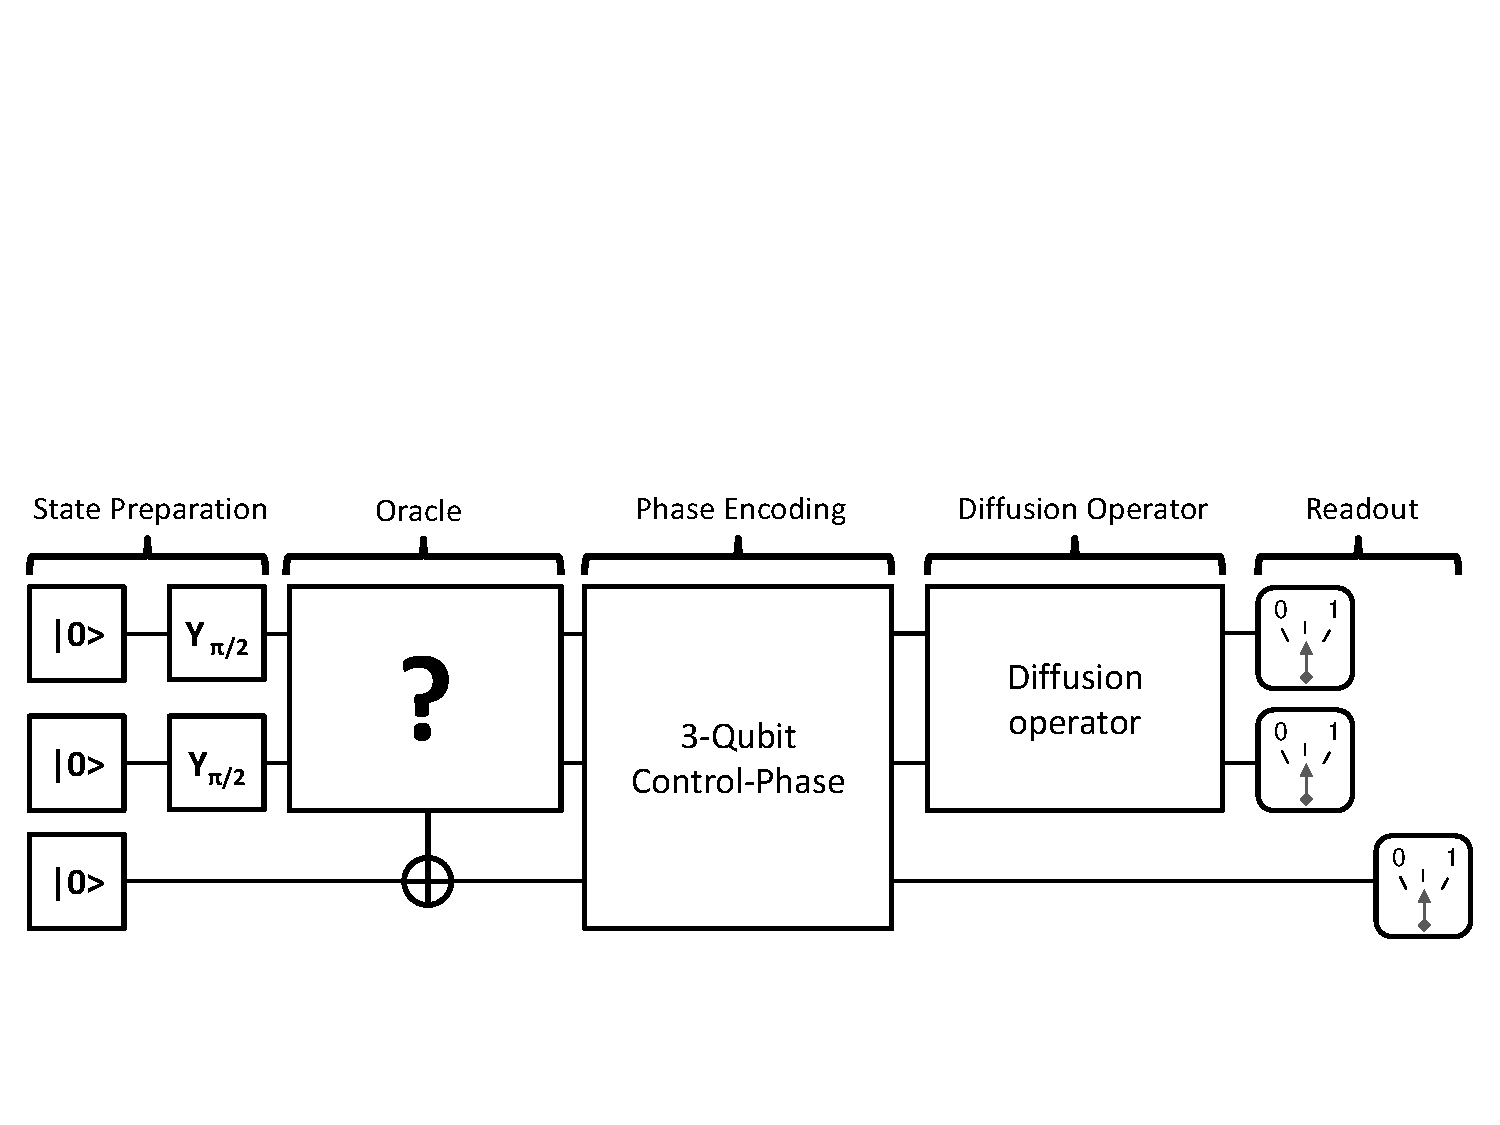
\includegraphics[width=1\textwidth]{./material/papers/grover/quantum_algorithm_full}
	\caption[Full version of an implementation of the two-qubit Grover search algorithm]{A full version of an implementation of the two-qubit Grover search algorithm. This algorithm works on a two-qubit input state and flips the state of a control qubit for one of the four possible input states in accordance to an unknown Oracle function. It then applies a 3-qubit control-phase operation of that maps $\ket{xx1}\to -\ket{xx1}$, $\ket{xx0}\to\ket{xx0}$ to encode the state of the control qubit directly in the two input qubits and then uses a diffusion operator to determine the state which has been marked by the Oracle function.}
	\label{fig:GroverAlgorithmFullSchematic}
\end{figure}

\smallskip

Fig. \ref{fig:GroverAlgorithmFullSchematic} shows a full ancilla-based implementation of the two-qubit Grover algorithm using the quantum Oracle function described above. This algorithm proceeds almost identically to version of the Grover algorithm discussed in the last section, with the only difference that after calling the Quantum oracle function it uses a three-qubit control-not (CNOT) gate $C$ of the form

\begin{equation}
C = \mathrm{I}^{n\otimes n}-2\sum\limits_{ij} \ket{ij1}\bra{ij1}
\end{equation}

to phase-encoded the state of the anciall qubit into the state of the input qubit register. During the further operation of the algorithm, the ancilla qubit must not be read out since it will destroy the prepared state of the input qubit register otherwise. However, reading out the value of the ancilla qubit after the end of the algorithm allows one to check for the existence of a solution of the search problem, in which case the ancilla qubit will return a value of $\ket{1}$ upon readout.

\section{Comparision to a Classical Algorithm}

\begin{figure}[ht!]
	\centering
		\includegraphics[width=1.0\textwidth]{"./material/papers/grover/classical_reversible_algorithm"}
	\caption{Classical reversible implementation of a search algorithm on a two-bit input register. The Oracle function can be implemented by two single-bit NOT operations and a Toffoli gate. R designates the generation of a random binary value at the beginning of the algorithm If the Oracle does not yield the correct answer, the test state gets incremented. The average success probability of the algorithm is 50 \%.}
	\label{fig:GroverClassicalReversibleAlgorithm}
\end{figure}

In order to quantify the quantum speed-up achieved for a certain quantum algorithm, it is necessary to formulate the problem solved by the quantum algorithm such that it can be compared to an equivalent problem that can be solved by a classical algorithm. The classical search problem solved by the Grover search algorithm has already been discussed in the first section of this chapter and with the ancilla-based version of the Grover algorithm that we introduced in the last section it is possible to directly compare the performance of a classical search algorithm with that of the Grover search algorithm. As has been discussed above, any possible Oracle function can be implemented both in quantum computing as well as classical computing using reversible logic gates such as the Toffoli gate and the single-(qu)bit NOT gate. Using this fact, we can devise a simple probabilistic algorithm that solves our search algorithm. This algorithm is shown in fig. \ref{fig:GroverClassicalReversibleAlgorithm} and achieves a success probability of 50 \% by evaluating the function $\Or$ for a randomly generat two-qubit input value $r$. If $\Or(r)=1$, the algorithm directly returns $r$, otherwise it binary adds $1$ to the state $r$ and returns this incremented input state. By this technique, it achieves an average success probability of 50 \% over all four possible Oracle functions. This 50 \% success rate therefore provide a benchmark against which we will measure the speed-up of our implementation of the Grover algorithm.


\section{Experimental Implementation}

\begin{figure}[ht!]
	\centering
		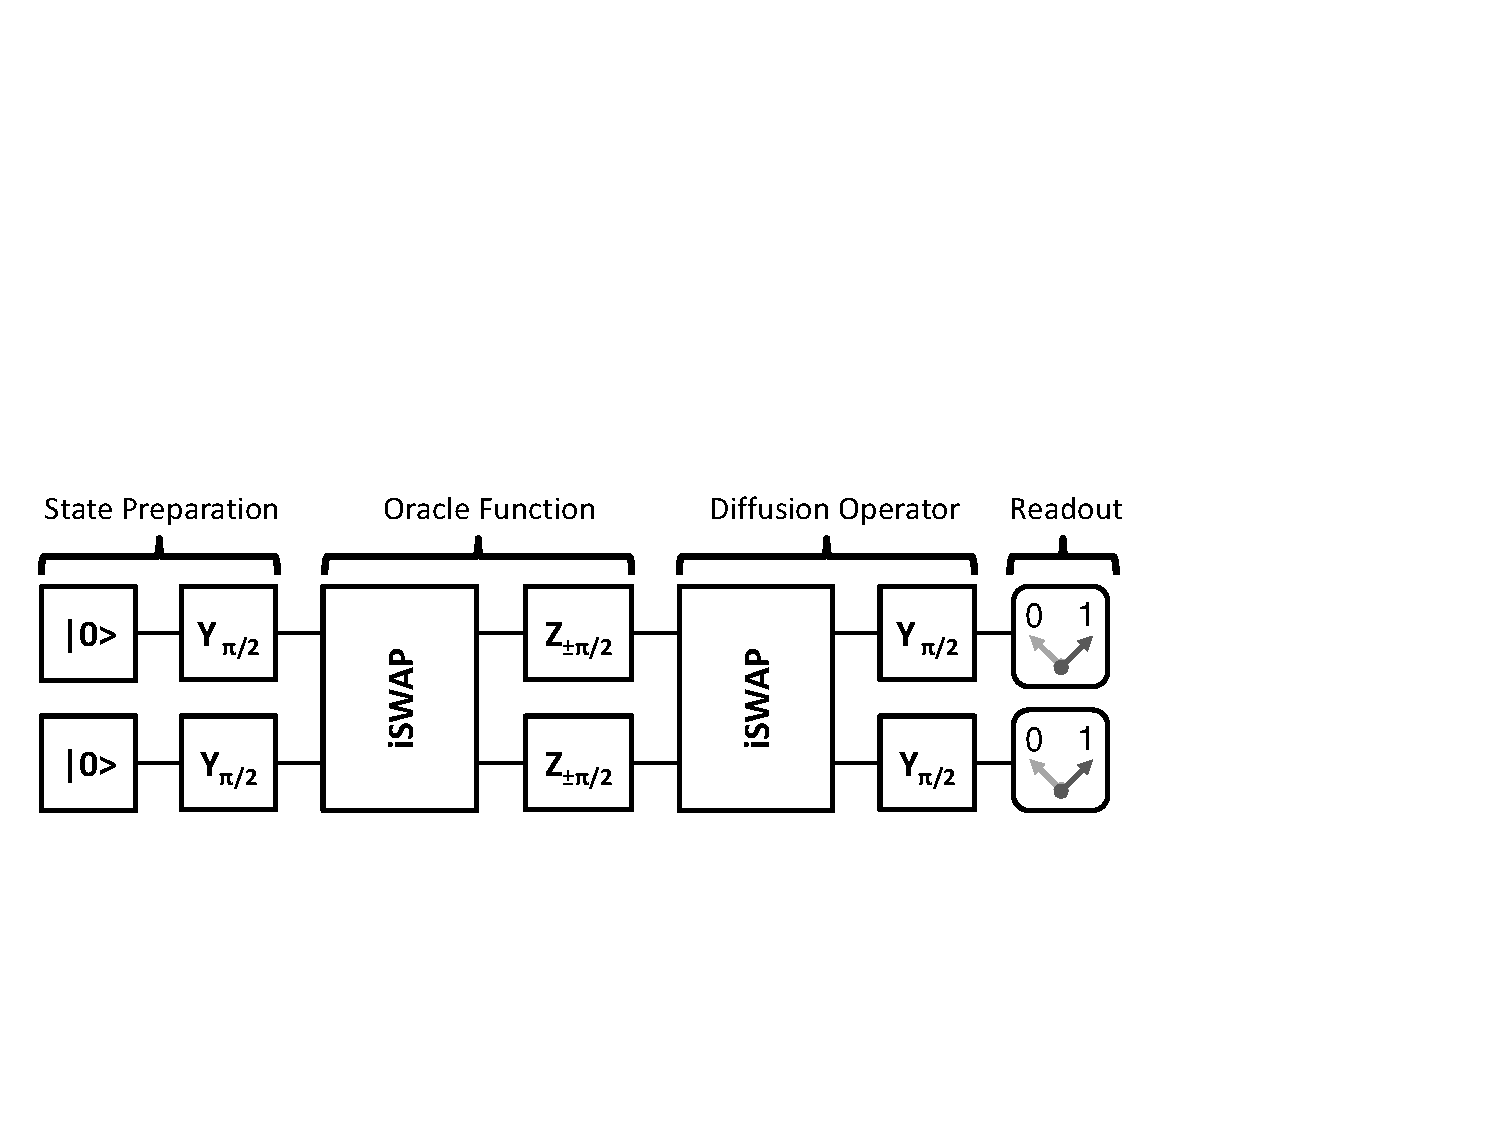
\includegraphics[width=0.8\textwidth]{./material/papers/grover/grover_algorithm}
	\caption[Schematic of our implementation of the Grover search algorithm]{Schematic of our implementation of the Grover search algorithm. The algorithm consists in generating a fully superposed input state, applying the Oracle function to it and analyzing the resulting state by applying the Diffusion transform to it and reading out the value of the qubit register afterwards.}
	\label{fig:GroverAlgorithmSchematic}
\end{figure}

In this work we implement a compiled version of the two-qubit Grover algorithm. The gate sequence of the algorithm is shown in fig. \ref{fig:GroverAlgorithmSchematic} and consists in two $i\mathrm{SWAP}$ gates and six single-qubit gates applied to an initial state $\ket{00}$. The first $i\mathrm{SWAP}$ gate together with the two single-qubit $Z_{\pm \pi}$ rotations implements the Oracle function $f(x)$ as given in eq. (\ref{eq:GroverOracleFunction}), where the signs of the rotation operations determines the state which is marked and can be either $\ket{00}$ (corresponding to a $Z^1_{-\pi/2}\cdot Z^2_{-\pi/2}$ rotation), $\ket{01}$ ($Z^1_{-\pi/2}\cdot Z^2_{\pi/2}$), $\ket{10}$ ($Z^1_{\pi/2}\cdot Z^2_{-\pi/2}$) or $\ket{11}$ ($Z^1_{\pi/2}\cdot Z^2_{\pi/2}$). The second $i\mathrm{SWAP}$ operation together with the following $X^1_{\pi/2}\cdot X^2_{\pi/2}$ operation implements the difussion operator as given by eq (\ref{eq:GroverDiffusionOperator}). The final step of the algorithm consists in reading out the two-qubit register.

\subsection{Pulse Sequence}

To implement the gate sequence described above we need to realize a sequence of microwave and flux pulses which realize the individual quantum gates of the sequence. To eliminate possible gate errors, we perform a series of calibration measurements before to tune-up the individual single- and two-qubit gates needed for the algorithm. In addition, we run individual parts of the algorithm successively and perform quantum state tomography to characterize the state of the quantum register after each step of the algorithm and correct the gate operations applied to the qubit in order to maximize the fidelity of the measured states in respect to the ideal ones. Fig. \ref{fig:GroverPulseSequence} shows an experimental pulse sequence for the Grover algorithm with an Oracle operator marking the state $\ket{00}$. Shown are the frequencies of the two qubits during the runtime of the algorithm and the microwave drive and readout pulses applied to them.

\begin{figure}[htb!]
	\centering
		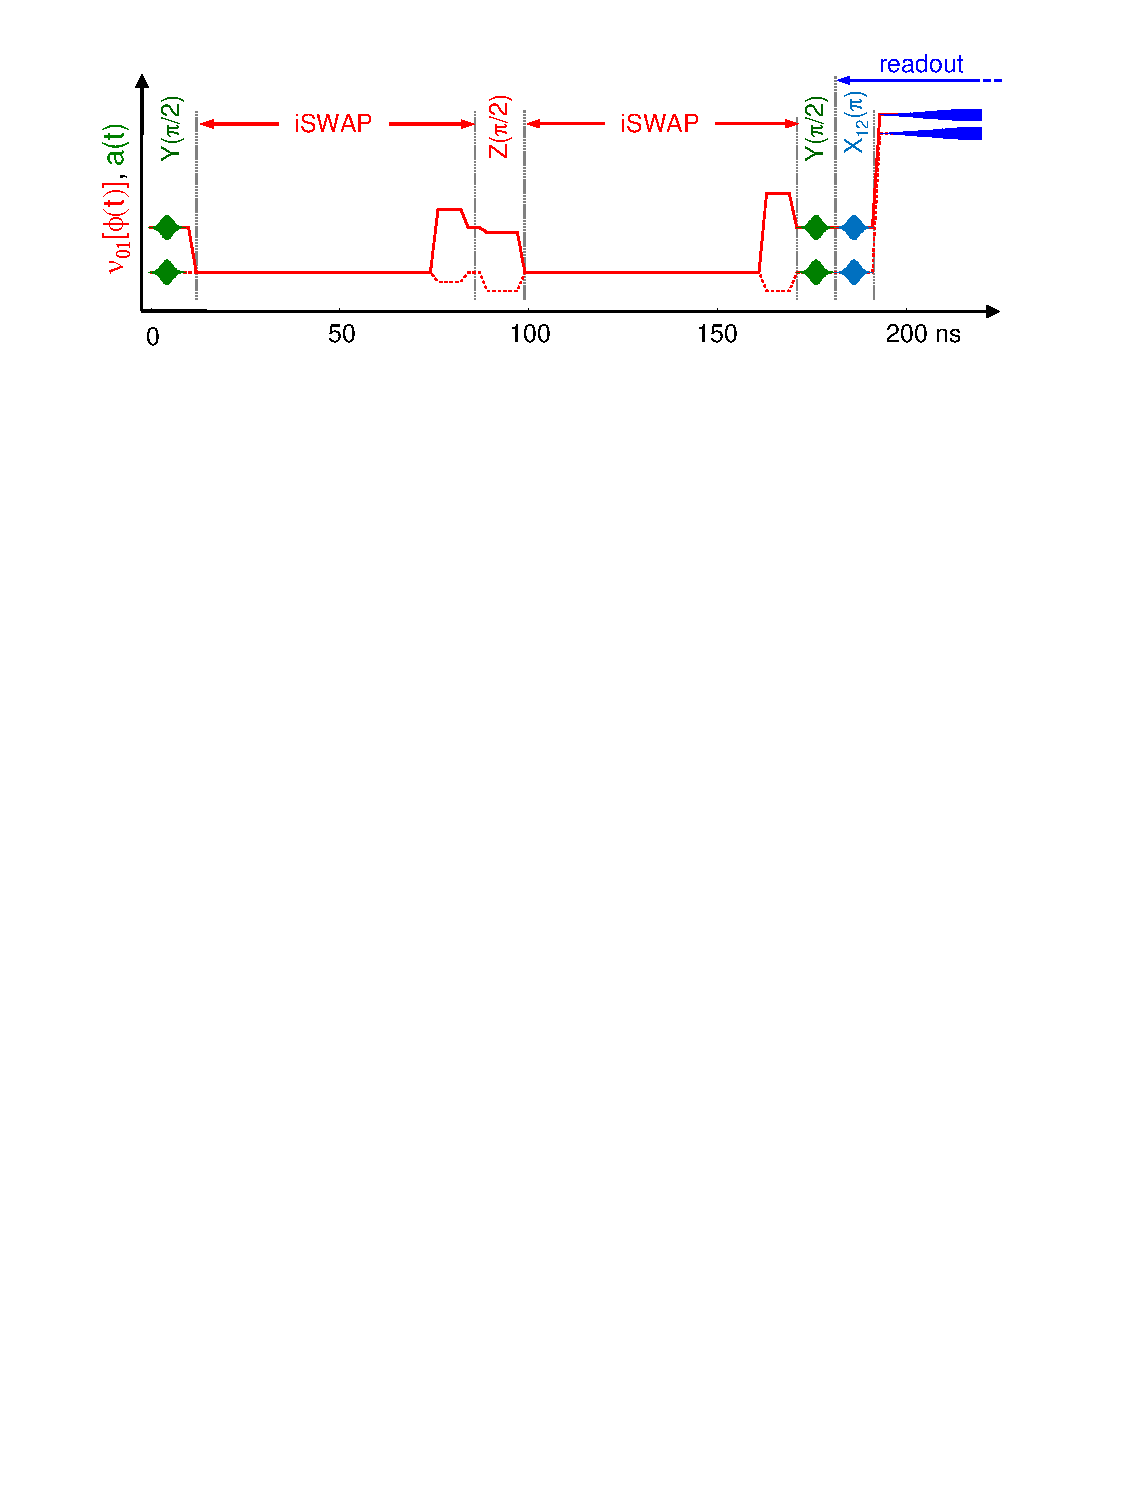
\includegraphics[width=1.\textwidth]{./material/papers/grover/figures/grover_algorithm_pulse_sequence}
	\caption[Pulse sequence used for implementing Grovers search algorithm]{The pulse sequence used in realizing Grover's quantum search algorithm. First, a $Y_{\pi/2}$ pulse is applied to each qubit to produce the fully superposed state $1/2(\ket{00}+\ket{01}+\ket{10}+\ket{11})$. Then, an $i\mathrm{SWAP}$ gate is applied, followed by a $Z_{\pm \pi /2}$ gate on each qubit, which corrsponds to the application of the oracle function. The resulting state is then analyzed using another $i\mathrm{SWAP}$ gate and two $Y_{\pi/2}$ gates to extract the state which has been marked by the oracle function. Optionally, a $Y^{12}_{\pi}$ pulse is used on each qubit to increase the readout fidelity.}
	\label{fig:GroverPulseSequence}
\end{figure}

\section{Results}

Here we'll discuss the results obtained when running the Grover search algorithm with our two-qubit processor. In the first section we'll analyze the quantum state of the qubit register during the algorithm by performing quantum state tomography. In the second section we will present and discuss the single-run results obtained in our experiment.

\subsection{State Tomography of the Algorithm}

Fig. \ref{fig:GroverAlgorithmExperimentalResults} shows the results when running the Grover search algorithm for the four possible Oracle functions. Shown are quantum state tomographies after each step of the algorithm and the single-run results obtained when measuring the qubit register after the final step of the algorithm. In subfigures  (a)-(d) The black outlined circles in the density matrices represent the ideal theoretical states, whereas the colored, solid circles represent the experimentially measured states. The trace fidelities of all states with the ideal ones are noted above each density matrix. As can be seen, the fidelity diminshes as a function of the runtime of the algorithm due to dephasing and relaxation of the qubit register. The experimental single-shot probabilities in subfigure (e) are shown along with the expected probabilities, which are calculated based on the readout matrix of our two-qubit system and the state tomographies after the final state of the algorithm. 

\begin{figure}[ht!]
	\centering
		\includegraphics[width=1.\textwidth]{"./data/ct5/2011_04_21 - grover and tomo/good_data/grover algorithm - single run results - density matrices only"}
	\caption[Quantum state tomographies at different steps during the Grover search algorithm and single-run outcome probabilities]{Quantum state tomographies at different steps of the Grover search algorithm and single-run outcome probabilities. The density matrices show the experimentally measured states in color and the theoretical states in black. For each state, the trace fidelity $F_{tr}(\rho_A,\rho_B) = \mathrm{Tr}\{\rho_A\cdot\rho_B\}$ is shown above the density matrix.}
	\label{fig:GroverAlgorithmExperimentalResults}
\end{figure}

\subsection{Single Run Results}

\begin{figure}[ht!]
	\centering
		\includegraphics[width=1.\textwidth]{"./data/ct5/2011_04_21 - grover and tomo/good_data/grover algorithm - single run probabilities"}
		\caption[Single-run success probabilities of the Grover search algorithm]{The single-run success probabilities of our implementation of the Grover search algorithm. Shown are the averaged probabilities for the four possible Oracle functions. The red bars correspond to measured values, the blue ones to expected probabilities calculated using the reconstructed density matrices after the final step of the algorithm and the measured two-qubit readout matrix. The dashed line indicates the average success probability of a classical query-and-guess algorithm for comparision.}
	\label{fig:GroverSingleShotResults}
\end{figure}

The experimental state tomographies discussed in the last section show that we are able to implement the Grover search algorithm with adequate fidelity using our two-qubit processor. However, the analysis of the two-qubit register by quantum state tomography at the end of the algorithm does not prove that we can achieve real quantum speed-up with our processor. For this, it is necessary to directly read out the state of the qubit register at the end of the algorithm {\it without} performing any kind of error correction afterwards. By looking at this ``raw'' outcome data and averaging it over many identical runs of the processor we can then quantify the success rate and the fidelity of the algorithm we implemented. The results of such measurements that we performed for the four possible Oracle functions is shown in fig. \ref{fig:GroverSingleShotResults}. There, the different plots represent averaged outcome probabilities when measuring the state of the two-qubit register after performing the Grover algorithm, shown for all four possible Oracle functions. For comparision, we also show the expected outcome probabilities that are calculated based on the quantum state tomographies discussed above and the readout matrix of the two-qubit system. As can be seen, the agreement between the measured and calculated probabilities is quite good. The dashed line in all plots corresponds to the success probability of a classical ``query-and-guess'' algorithm, which is bound to 50 \% and is therefore the benchmark for quantum speed-up in this system. As can be seen, our implementation of the Grover search algorithm outperforms a classical search algorithm for all four Oracle functions.

\section{Algorithm Fidelity}

We can define the average fidelity of the algorithm in a single run, which corresponds to the averaged success probabilities measured for all four Oracle functions and averaged over a large sample set. Table \ref{tab:Probabilities-for-obtaining} shows these single-run probabilities along with the so-called {\it user fidelities}, which are given as

\begin{equation}
f_{ab} = p(\ket{ab}|ab) = \frac{p(ab |\ket{ab})}{\sum\limits_{uv}p(uv|\ket{uv})} 
\end{equation}

and correspond to the probability of having obtained the correct answer given a certain outcome, averaged over all four possible Oracle functions. For all four, both the single-run and user fidelities are $> 50 \%$, hence providing a quantum speed-up in comparision with a classical query-and-guess algorithm.

\begin{table}[H]
\begin{centering}
\begin{tabular}{|c|c|c|c|c|c|c|}
\hline 
$ab$/$|uv\rangle$ & $\left|00\right\rangle $ & $\left|01\right\rangle $ & $\left|10\right\rangle $ & $\left|11\right\rangle $ & $\sum$ & $f_{ab}$\tabularnewline
\hline
\hline 
00 & \textcolor{red}{0.666} & 0.192 & 0.188 & 0.122 & 1.168 & 57.0 \%\tabularnewline
\hline 
01 & 0.127 & \textcolor{red}{0.554} & 0.071 & 0.122 & 0.874 & 63.4 \%\tabularnewline
\hline 
10 & 0.128 & 0.106 & \textcolor{red}{0.615} & 0.239 & 1.088 & 56.5 \%\tabularnewline
\hline 
11 & 0.079 & 0.148 & 0.126 & \textcolor{red}{0.517} & 0.870 & 59.4 \%\tabularnewline
\hline
\end{tabular}
\par\end{centering}

\caption{\label{tab:Probabilities-for-obtaining}Conditional probabilities
$p_{ab/|uv\rangle}$ and statistical fidelities $f_{ab}$ for all
possible outcomes $ab$, measured for our version of Grover's algorithm.}

\end{table}

\section{Error Analysis}

There are three kind of errors arising in our implementation of the Grover search algorithm which we will analyze in the following section. These errors are:

\begin{enumerate}
	\item Deterministic, unitary gate errors arising in the algorithm
	\item Stochastic errors introduced due to qubit decoherence during the runtime of the algorithm.
	\item Readout errors due to qubit relaxation during the readout of the qubit state, insufficient coupling between the qubit and the readout or retrapping of the readout state during latching.
\end{enumerate}

\subsection{Gate Errors \& Decoherence}

Gate errors are unitary errors that arise due to misshaped or mistuned gate pulses. Usually the effect of these errors is combined with stochastic, non-unitary error sources arising due to qubit decoherence during the runtime of the algorithm. To quantify these errors we generate a model of our algorithm where we take into account both unitary as well as non-unitary error sources and perform numerical optimization of the error parameters to generate a quantitative model. We repeat this procedure for all four algorithm runs corresponding to the different Oracle functions.

\subsubsection{Decoherence}

Usually we can model decoherence processes in our algorithm either by integrating an effective master equation. For our error model, however, we chose to use a set of discrete decoherence operators that model amplitude (i.e. $T_1$) and phase daming (i.e. $T_\phi$) processes. We can model the decoherence in our algorithm by applying these operators to the calculated quantum states after each individual step of the algorithm, taking into account the experimental runtime of the step. By this we can generate an error model incorporating the most relevant experimental decoherence processes without needing to numerically integrate a Lindblad equation, thereby greatly speeding up the paramter fitting.

\smallskip

The single-qubit operators describing amplitude-daming (i.e. energy relaxation) of the qubit state are given as \citep{michael_a._nielsen_quantum_2000}

\begin{align}
 E_1^{T_1} & = \left(\begin{array}{cc} 1 & 0 \\ 0 & \sqrt{1-\gamma_{T_1}} \end{array}\right)   &  E_2^{T_1}  & = \left( \begin{array}{cc} 0 & \sqrt{\gamma_{T_1}} \\ 0 & 0 \end{array} \right) \label{eq:grover_energy_relaxation}
\end{align}

The phase-daming (i.e. dephasing) operators can be written as

\begin{align}
 E_1^{T_{\phi 1}} & = \left(\begin{array}{cc} 1 & 0 \\ 0 & \sqrt{1-\gamma_\phi} \end{array}\right)   &  E_2^{T_{\phi 1}}  & = \left( \begin{array}{cc} 0 & 0 \\ 0 & \sqrt{\gamma_\phi}  \end{array} \right) \label{eq:grover_phase_decoherence}
\end{align}

Both operators are applied to $\rho$ according to

\begin{equation}
\rho \to E_1 \rho E_1^\dagger+E_2 \rho E_2^\dagger
\end{equation}

and result in a trace-preserving, non-unitary evolution of the quantum state of $\rho$. The decoherence factors $\gamma$ in the operators can be calculated from the corresponding relaxation and dephasing rates as $\gamma_{T_{1,2}}(t) = 1-\exp{\left(-t \Gamma_{1,2}^{T_1}\right)}$ and $\gamma_{\phi_{1,2}} = 1-\exp{\left(-t \Gamma_{1,2}^{T_\phi}/2\right)}$, where $t$ is the time during which the state is exposed to the decoherence process.

\smallskip

\begin{figure}[ht!]
	\centering
		\includegraphics[width=0.85\textwidth]{"./material/papers/grover/grover_error_model"}
	\caption[Error model used for analyzing gate and decoherence errors for the Grover search algorithm]{The error model we use to analyze the different gate and decoherence errors present when running the Grover search algorithm. The dotted lines indicate the points at which the quantum state has been measured by state tomography. Zigged arrows indicate the decoherence present in the system.}
	\label{fig:GroverErrorModel}
\end{figure}


The full error model that we use to model the algorithm is shown in fig. \ref{fig:GroverErrorModel}. In this model, we take into account the following errors

\begin{itemize}
 \item {\bf Energy relaxation and phase decoherence}: We model energy relaxation and phase relaxation of our qubit by using the processes given in eqs. (\ref{eq:grover_energy_relaxation}) and (\ref{eq:grover_phase_decoherence}), applying the energy relaxation operator after each step of the algorithm, taking into account gate time of the performed operation.
 \item {\bf Single-qubit gate errors}: We model rotation angle and rotation phase errors of our single-qubit $X_\alpha$ and $Y_\alpha$ gates by replacing them with operators of the form $X_\alpha\to \phi_{\alpha'} = \cos{\phi}X_{\alpha'}+\sin{\phi}Y_{\alpha'}$ and $Y_\alpha \to \varphi_{\alpha'} = \sin{\varphi}X_{\alpha'}+\cos{\varphi}Y_{\alpha'}$. For $Z$-type single-qubit operators we model only rotation angle errors by replacing $Z_\alpha \to Z_{\alpha'}$ 
 \item {\bf Two-qubit gate errors:} We model both detuning and gate-length errors of our $i\mathrm{SWAP}$ 2-qubit gates.
\end{itemize}

The evolution operator of a detuned iSWAP operation is given as

\begin{equation}
i\mathrm{SWAP}(t,\Delta) = \left(
			\begin{array}{cccc}
				1 & 0 & 0 & 0 \\
				0 & \cos{t g_{e}}-i\frac{\Delta}{g_{e}}\sin{t g_{e}} & i \frac{g}{g_e}\sin{t g_{e}} & 0 \\
				0 & i\frac{g}{g_e}\sin{t g_{e}} & \cos{t g_{e}}+i\frac{\Delta}{g_{e}}\sin{t g_{e}} & 0 \\
				0 & 0 & 0 & 1 \\
			\end{array}
	\right) \label{eq:swap_with_detuning}
\end{equation}

\begin{figure}
	\centering
		\rotatebox{90}{\includegraphics[width=1.2\textwidth]{"./data/ct5/2011_04_21 - grover and tomo/good_data/grover - simulated density matrices with errors"}}
	\caption[Quantum state tomographies at different steps during the Grover search algorithm and single-run outcome probabilities]{Quantum state tomographies at different steps of the Grover search algorithm and single-run outcome probabilities. The density matrices show the experimentally measured states in color and the theoretical states in black. For each state, the trace fidelity $F_{tr}(\rho_A,\rho_B) = \mathrm{Tr}\{\rho_A\cdot\rho_B\}$ is shown above the density matrix.}
	\label{fig:grover_error_model}
\end{figure}

where $g_e = \sqrt{g^2+\Delta^2}$ is the effective swap frequency at a qubit frequency detuning $f_{01}^1-f_{01}^2 = 2\Delta$. Often it is pratical to replace $t$ and $\Delta$ with $\beta = t g_{e}$ and $\delta = \Delta / g$. Using this notation of the iSWAP gate and the definition of the single-qubit gates as discussed before, the full algorithm with gate errors can be written as (for right-multiplication)

\begin{equation}
\mathrm{Grover} = \phi_{\gamma_1}^1\otimes \phi_{\gamma_2}^2\cdot i\mathrm{SWAP}(\epsilon_2,\delta_2)\cdot Z_{\beta_1}\otimes Z_{\beta_2}\cdot i\mathrm{SWAP}(\epsilon_1,\delta_1)\cdot\varphi_{\alpha_1}^1\otimes \varphi_{\alpha_2}^2 \label{eq:grover_error_model}
\end{equation}

In addition, we add a dephasing and relaxation error after each step of the algorithm to simulate the decoherence during the executing. Numerical optimization is used to produce a fit of all the gate error parameters, which is shown in tab. \ref{tab:grover_error_parameters}. The qubit relaxation and dephasing times have been measured independently and are not part of the fit.

\begin{table}[ht!]
\centering
\footnotesize{
\begin{tabular}{r|rrrrrrrrrrrrrr}
state & $\delta_1$ & $\delta_2$ & $\alpha_1$ & $\alpha_2$ & $\varphi_1$ & $\varphi_2$ & $\epsilon_1$ & $\beta_1$ & $\beta_2$ & $\epsilon_2$ & $\gamma_1$ & $\gamma_2$ & $\phi_1$ & $\phi_2$ \\ \hline
$\ket{00}$ & 0.06 & -0.06 & -2.5 & 2.7 & 6.1 & 3.1 & -7.3 & -3.3 & -4.1 & 7.5 & 29 & 9.3 & 0.66 & -1.7
 \\
$\ket{01}$ & 0.04 & -0.3 & -0.1 & 0.1 & 7.9 & 3.6 & -11 & -5.9 & 2.2 & -6.9 & 28 & -19 &  9 &  2
 \\
$\ket{10}$ & 0.09 & -0.2 & -3.1 & 1.7 &  1 & -2.5 & -6.5 & -15 & -22 & -7.5 & -15 & 32 & 3.6 & 5.2
\\
$\ket{11}$ & 0.16 & 0.13 & -6 & 3.9 & 2.2 & 0.9 & -9.5 & -20 & -15 & 17 & -12 & -32 & -7 & -8.9
\end{tabular}
}
\caption[Fitted gate error parameters of the Grover algorithm]{Fitted error parameters for the measured density matrices, modeled according to the error model given in eq. (\ref{eq:grover_error_model}). Alle angles are given in $\deg$.}
\label{tab:grover_error_parameters}
\end{table}

The results of the fitted error model are shown in tab. \ref{tab:grover_error_parameters}. As can bee seen, the phase and gate-time errors for the first gates are comparatively small and grow bigger during the following steps of the algorithm. The phase errors are bigger for the states $\ket{10}$ and $\ket{11}$, as are the gate-length errors for the two $i\mathrm{SWAP}$ gates used in the algorithm.

\smallskip

Fig. \ref{fig:grover_error_model} shows again the measured density matrices for our realization of the Grover search algorithm, this time overlaid with the numerically optimized error model according to eq. (\ref{eq:grover_error_model}). As can be seen, our error model is able to capture most of the observed experimental errors and to reproduce to a very good accuracy the observed density matrices. The state fidelities according to eq. \ref{eq:state_fidelity} between the measured density matrices and those of the fitted error model are shown above each density matrix.

\subsubsection{Fidelity of the Oracle and diffusion operators}

It is interesting to analyze the individual fidelity of the Oracle and diffusion operators that make up the Grover algorithm. For this, we compare the action of the ideal operators $D'$ and $R'$ with that of the experimentally implemented versions $D'_{e}$ and $R'_{e}$, taking the measured quantum states before applying each of the operators as input. We take as the fidelity of each operator the average state fidelity of the measured output states as compared to the calculated ones, such that

\begin{eqnarray}
F(D'_{e}) & = & F(D'\rho_{in}D^{'\dagger},D'_e \rho_{in} D_{e}^{'\dagger}) \label{eq:grover_diffusion_fidelity} \\
F(R'_{e}) & = & F(R'\rho_{in}R^{'\dagger},R'_e \rho_{in} R_{e}^{'\dagger}) \label{eq:grover_oracle_fidelity}
\end{eqnarray}

where we also use the state fidelity according to eq. \ref{eq:state_fidelity}. By this method, we obtain the following fidelities for the two gate operations:

\begin{table}[ht!]
\centering
\begin{tabular}{r|rrrr|l}
Operator / State & $\ket{00}$ & $\ket{01}$ & $\ket{10}$ & $\ket{11}$ & Average \\ \hline 
$D'$ & 92.3 & 93.4 & 94.3 & 91.7 & 92.9 \\
$R'$ & 94.5 & 93.6 & 88.5 & 87.7 & 91.1
\end{tabular}
\caption[Measured fidelities of the quantum Oracle and diffusion operators used in the Grover search algorithm]{Measured fidelities of the quantum Oracle and diffusion operators used in the Grover search algorithm according to eqs. (\ref{eq:grover_diffusion_fidelity}) and (\ref{eq:grover_oracle_fidelity}). All fidelities are given in percent.}
\end{table}

\subsection{Readout Errors}

\begin{figure}[ht!]
	\centering
\includegraphics[width=0.19\textwidth]{"./data/ct5/2011_04_21 - grover and tomo/good_data/single qubit readouts"}
\includegraphics[width=0.79\textwidth]{"./data/ct5/2011_04_21 - grover and tomo/good_data/readout and crosstalk - 2 plots"}
	\caption[Measured single- and two-qubit readout matrices and crosstalk matrix for the Grover search algorithm experiment]{a.)The measured single-qubit readout matrices, showing the readout outcome probabilities as a function of the prepared state for both qubits. b.)The measured two-qubit readout matrix, showing again the detector outcome probabilities versus the prepared qubit states. c.) The crosstalk matrix, corresponding to the product of the two-qubit readout matrix and the Kronecker product of the single-qubit readout matrices. Note that the $\ket{1}\to\ket{2}$ shelving method is used for reading out the qubit state, which increases readout fidelity but also inter-qubit readout crosstalk.}
	\label{fig:GroverReadoutMatrix}
\end{figure}

Another source of errors arises due to the imperfection of our qubit readout. Mostly, qubit relaxation during the readout process reduces the visibility of individual qubit states and introduces errors when reading out the qubit register in the final step of the algorithm. We can easily quantify those readout errors by using the readout matrix that was introduced in the last chapter. When running the Grover algorithm we use the $\ket{1}\to\ket{2}$ shelving method described in the last chapter to increase the readout contrast and thereby the algorithm fidelity. This technique reduces single-qubit readout errors but increases inter-qubit readout crosstalk. To quantify all single-qubit and inter-qubit readout errors, we first model the readout matrix $R$ of the two-qubit system as a product $R=R_{v}\cdot R_{ct}$, where $R_{v}$ is the so-called {\it visibility matrix} and $R_{ct}$ a matrix describing the readout crosstalk. The visibility matrix can be written as the Kronecker product $R_{v} = R_{v}^1 \otimes R_{v}^2$ of the two single-qubit readout matrices, which have the form

\begin{equation}
R_{v}^{1,2} = \left(
			\begin{array}{cc}
				p_{00}^{1,2} & 1-p_{11}^{1,2} \\
				1-p_{00}^{1,2} & p_{11}^{1,2}
			\end{array}
		\right)
\end{equation}

Here, $p_{00}^{1,2}$ ($p_{11}^{1,2}$) corresponds to the probability to measure the value $0$ ($1$) at the readout after having prepared the qubit in state $\ket{0}$ ($\ket{1}$). Usually, the full two-qubit readout matrix $R$ and the single-qubit readout matrices $R_{v}^{1,2}$ are measured experimentially which allows us then to calculate the crosstalk matrix as $R_{ct} = R_{v}^{-1}\cdot R$. The three matrices measured in our experiment are shown in fig. \ref{fig:GroverReadoutMatrix}. As can be seen, the single-qubit readout fidelities range between 87 - 96 \% and the combined two-qubit readout fidelities between 75 - 85 \%. Depending on the qubit state we also observe between 3-5 \% inter-qubit readout crosstalk in our system.

\smallskip

Fig. \ref{fig:GroverAlgorithmExperimentalResults}e shows the single-run probabilities when running the Grover algorithm for the four different Oracle functions. In blue, the expected readout outcome probabilities, as calculated using the state tomography of the final states given in fig. \ref{fig:GroverAlgorithmExperimentalResults}d and the measured readout matrix of our system are shown along the measured readout outcome probabilities. The readout error model shows good quantitative agreement with the measured data, with deviations most probably due to parameter drifts occured between the measurment of the quantum state tomography and the single-run experiment.

\section{Conclusions}

To summarize, we have shown that we can implement the Grover search algorithm with our quantum processor and achieve a single-run fidelity that is sufficient to demonstrate simple probabilistic quantum speed-up as compared to a classical, reversible search algorithm. The error model formulated in this chapter is able to account for most of the observed imperfections and can explain the data we observed. The coherence times of our qubits does not permit the realization of more complex algorithm with this system, nevertheless it provides a proof-of-principle of our approach to build a superconducting quantum computer with individual-qubit single shot readout.

\smallskip

In the following chapter, we will discuss the extension of this approach to a system of four qubits and explain different strategies for scaling up such system to an even larger number of qubits.

%-Conclusions regarding quantum speed-up and applicability of results to larger-scale quantum computing.
